% The Experiments of the study should be laid out in a series of declarative paragraphs. Only results essential to establish the main points of the work should be included. Often the reporting of the results can be clearer if broken down into subsections. All figures and tables must be cited in the text and must be numbered in the order of their text citation. Figure legends should be self-explanatory, without referring to the text. They should identify the material that is being illustrated, what is shown, and its significance. Each table should be identified by number and should have a title. This section should not include long passages about the rationale of the experiments (which belong in the Introduction), or the methods used (which belong in the Material and Methods), nor should it include justification or discussion of the results (which belong in the Discussion section).
\chapter{Experiments}
\label{sec:experiments}

% We perform these experiments to showcase that we can indeed get semantically expressive creations with our proposed formulation.

\section{Initial Tests with CLIP}
\label{sec:clip-custom}

% Talk about the initial tests with CLIP that were motivated by the poor performance of CLIP on abstract images and sketches.
CLIP was trained on a large dataset of captioned natural images foraged from the internet.
While it generalizes well to many natural-image distributions and has proved to be a powerful zero-shot model for various tasks, it was not clear how well it would perform on sketches and abstract images. 

CLIP has been shown to not perform much better than chance on many tasks which were not well represented in its pre-training dataset.
% For example, it only achieved 88\% accuracy on the handwritten digits of MNIST.
The authors of CLIP also noted that it is particularly poor on tasks for fine-grained classification such as differentiating models of cars, species of flowers, and variants of aircraft.
It also struggles with more abstract and systematic tasks such as counting the number of objects in an image.

Moreover, \cite{vlmrm}, from their experiments with CLIP as a source of goal-conditioned rewards, reported that CLIP rewards are only meaningful and well-shaped for environments that are photorealistic enough for the CLIP visual encoder to interpret correctly.
They found that it is crucial to add textures and shading to the images to make them more realistic for CLIP to perform well.

Influenced by these observations and caveats, we suspected that our environments, since they are not photorealistic, might also be out-of-distribution. 
Yet, we expected them to be simple enough for CLIP to interpret correctly.

Thus, before testing our reward function, we conducted a series of simple experiments on the inference capabilities of CLIP on ShapeGridWorld and Tangram.
At the same time, there were several hyperparameters in the environments and CLIP into which we took insights with these initial tests.


\subsection{CLIP on Sketches and ShapeGridWorld}
\label{sec:clip-sketches}

We first tested CLIP on sketches of simple shapes from the ImageNet-Sketch dataset \citep{imagenet}.

We also compared these results with renderings of these sketches on ShapeGridWorld grids of different resolutions by registering them to a grid (see \secref{sec:sgw-registration} for more details on registration).
For an example, see \figref{fig:clip-sketches}.
\begin{figure}[h]
    \centering
    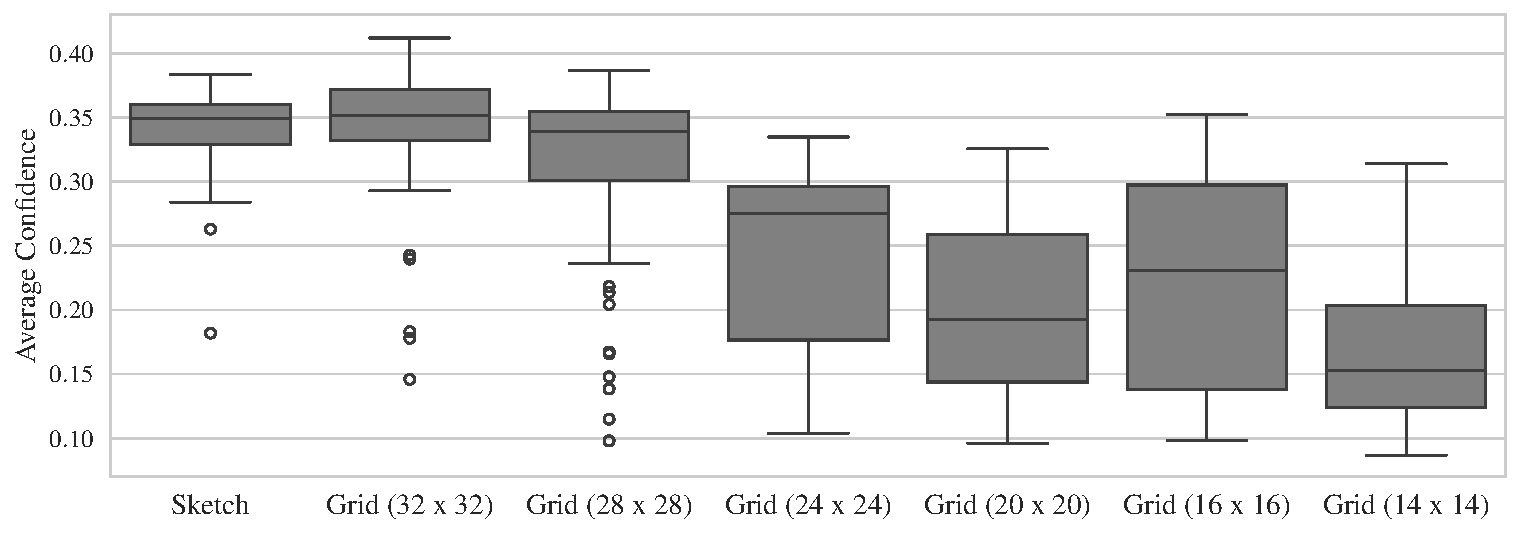
\includegraphics[width=\textwidth]{images/grid_comparison.pdf}
    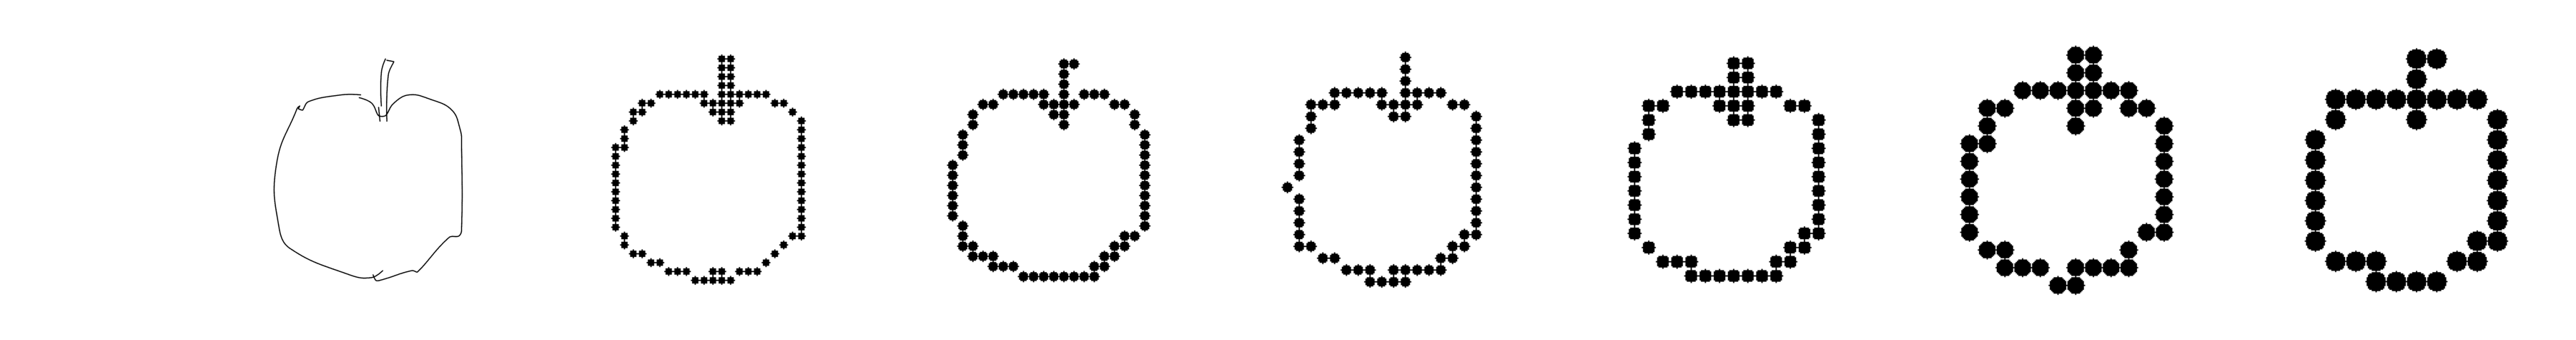
\includegraphics[width=\textwidth]{images/grid_comparison_images.png}
    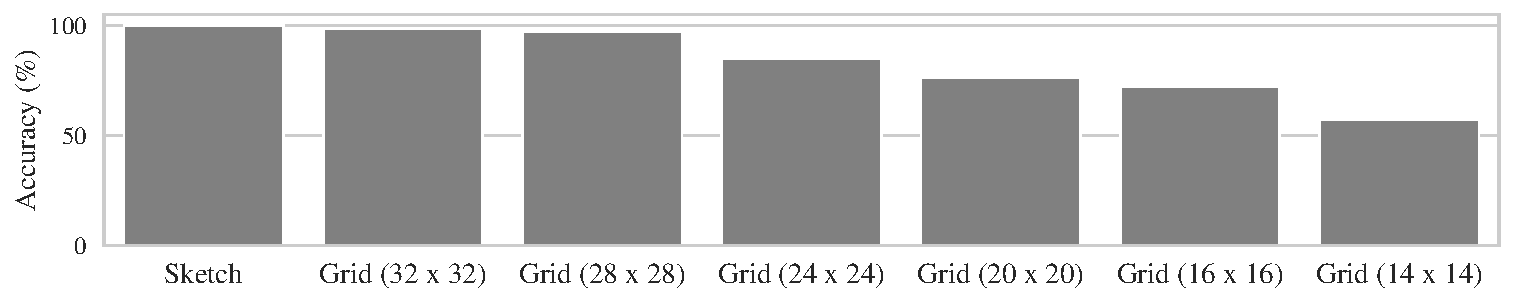
\includegraphics[width=\textwidth]{images/grid_comparison_accuracy.pdf}
    \caption[CLIP on sketches and ShapeGridWorld grids of different resolutions.]{CLIP on sketches and ShapeGridWorld grids of different resolutions.
    The first row shows the comparative similarity of the embeddings of \(80\) sketches of apples (and their grid counterparts) to the label ``sketch of an apple'' using the CLIP variant \texttt{ViT-L/14}.
    The probabilities are calculated using the equation \eqref{eq:clip-dist}, with temperature \(T = 1\), to show the trend.
    The categories for this example are ``apple'', ``chair'', ``car'', ``flower'', ``pencil'', ``house'', ``tree'', ``fish'', ``star'', and ``bird''.
    The middle row shows a sample of the images for each of the cases.
    The bottom row shows the accuracy (percentage of correct predictions) for each of the cases.
    }
    \label{fig:clip-sketches}
    % 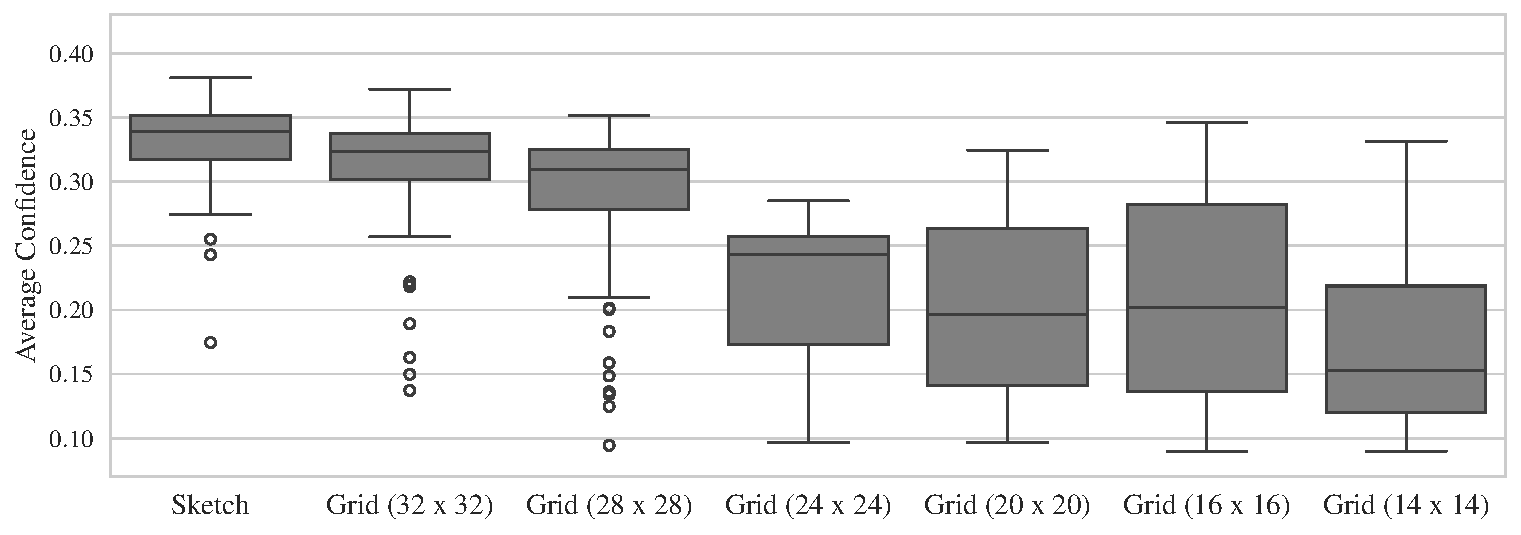
\includegraphics[width=\textwidth]{images/grid_comparison_inverted.pdf}
    % 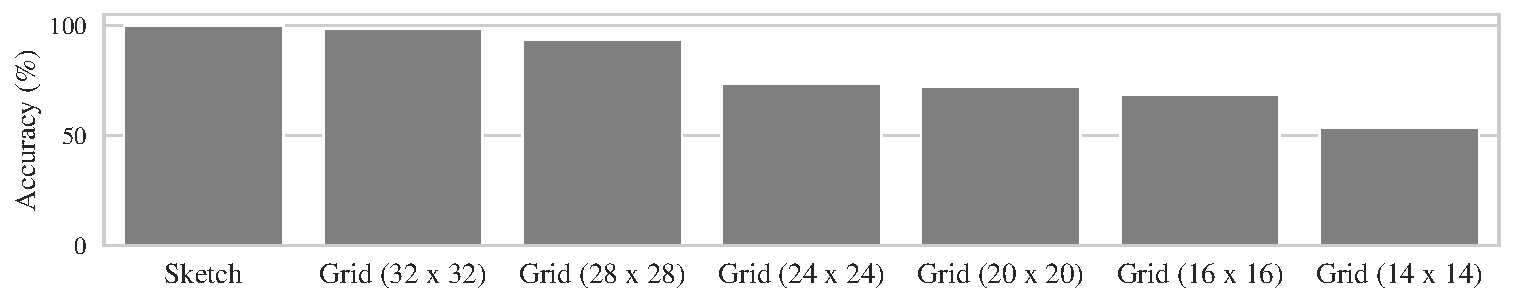
\includegraphics[width=\textwidth]{images/grid_comparison_accuracy_inverted.pdf}
    % \caption{CLIP on \emph{inverted} sketches and ShapeGridWorld grids of different resolutions.}
    % \label{fig:clip-sketches-inv}
\end{figure}
We found that CLIP can recognize these sketches quite well.
As the grid became coarser, the confidence and accuracy of CLIP decreased significantly.
For very coarse grids, the accuracy is almost as bad as random guessing.

We also experimented with inverting the images and found that results were consistently slightly better with black-on-white sketches (shown here) than with white-on-black sketches.
Yet, we did not notice any difference in performance with the addition of grayscale values in the pixel blocks in these experiments.

\begin{wrapfigure}[13]{r}{0.39\textwidth}
    \centering
    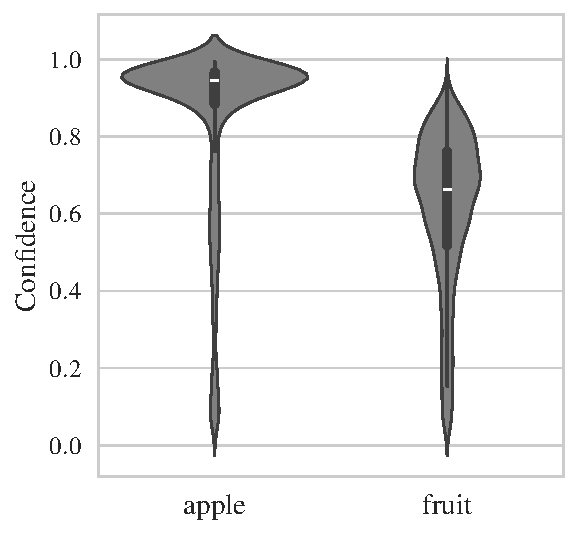
\includegraphics[width=0.36\textwidth]{images/hypercategory_comparison_2.pdf}
    \caption{CLIP on different levels of hypernymy and hyponymy of labels.}
    \label{fig:clip-hypercategory}
\end{wrapfigure}
In most cases, we also noticed that using specific labels like ``apple'' for a picture of an apple had better accuracy than using hypernyms like ``fruit'' (\figref{fig:clip-hypercategory}).

Additionally, we found that the bigger CLIP models performed better on these tasks than the smaller ones which is in line with observations from other studies on VLMs as a source of rewards, particularly \cite{vlmrm}.
We tried the same experiments with different sets of categories, prefixes, and suffixes; the results followed similar trends.

\subsection{CLIP on Tangram}
\label{sec:clip-tangram}

Tangram has fewer degrees of freedom than ShapeGridWorld and it is more abstract but it still allows for rich creative expression.
To test if it would be a feasible environment for our study, we used some images of creations on Tangram from the internet and used CLIP as a zero-shot classifier as above to test its performance using classes with simple Tangram creations.
We again found it to be quite good at recognizing these creations with good confidence.
\figref{fig:clip-tangram} shows a few examples.
\begin{figure}[h]
    \centering
    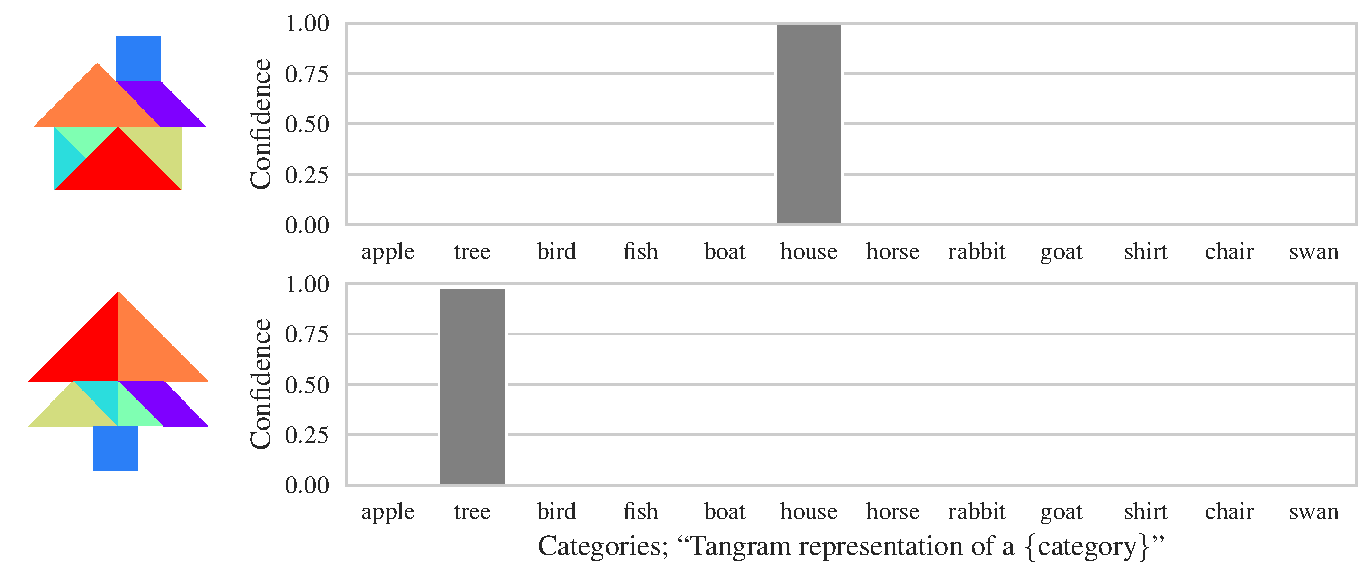
\includegraphics[width=\textwidth]{images/tangram_comparison_10.pdf}
    \caption{CLIP on a few simple Tangram creations.}
    \label{fig:clip-tangram}
\end{figure}

We did not find a significant trend in the effect of colors on the performance of CLIP, but inversions seemed to slightly affect the distribution of inferences in certain cases
(one such example is given in the appendix \figref{fig:clip-tangram-inversions}, where the distribution of CLIP was skewed in grayscale and white-on-black cases).
Consequently, we used colored or black-on-white binary renderings for our experiments.

More experiments on these hyperparameters are discussed in the later sections.


\section{Trajectory Analysis with Random Rollouts}
\label{sec:clip-problems}
% Problems with CLIP
Although we found that CLIP is quite good at recognizing these creations, we had to ensure that it would be a good source of rewards for our environments, or that the controller would be able to exploit it well to reach a sufficiently good local optimum.
To study the semantics entropy reward landscape, we conducted a series of experiments with random rollouts in the environments, i.e. starting from a meaningful creation, we perturbed the creation with randomly sampled actions and observed the effects on the reward.

These experiments showed that CLIP is quite susceptible to noise in its inferences, i.e. its probability distribution responds abruptly to small adjustments in the input image.
As a consequence of this, the reward is quite sparse, and more critically, there is a large semantic bias in not-so-meaningful images.
The sections below discuss these problems in detail.

\subsection{Sparse Rewards} % Sudden changes in rewards
\label{sec:sparse-rewards}

We observed that the inference of CLIP breaks suddenly with small changes in the image, i.e. its confidence in its classification is very sensitive.
This results in a sparse semantics entropy reward landscape.
\figref{fig:sparse-rewards} illustrates this problem.

\begin{figure}[h]
    \centering
    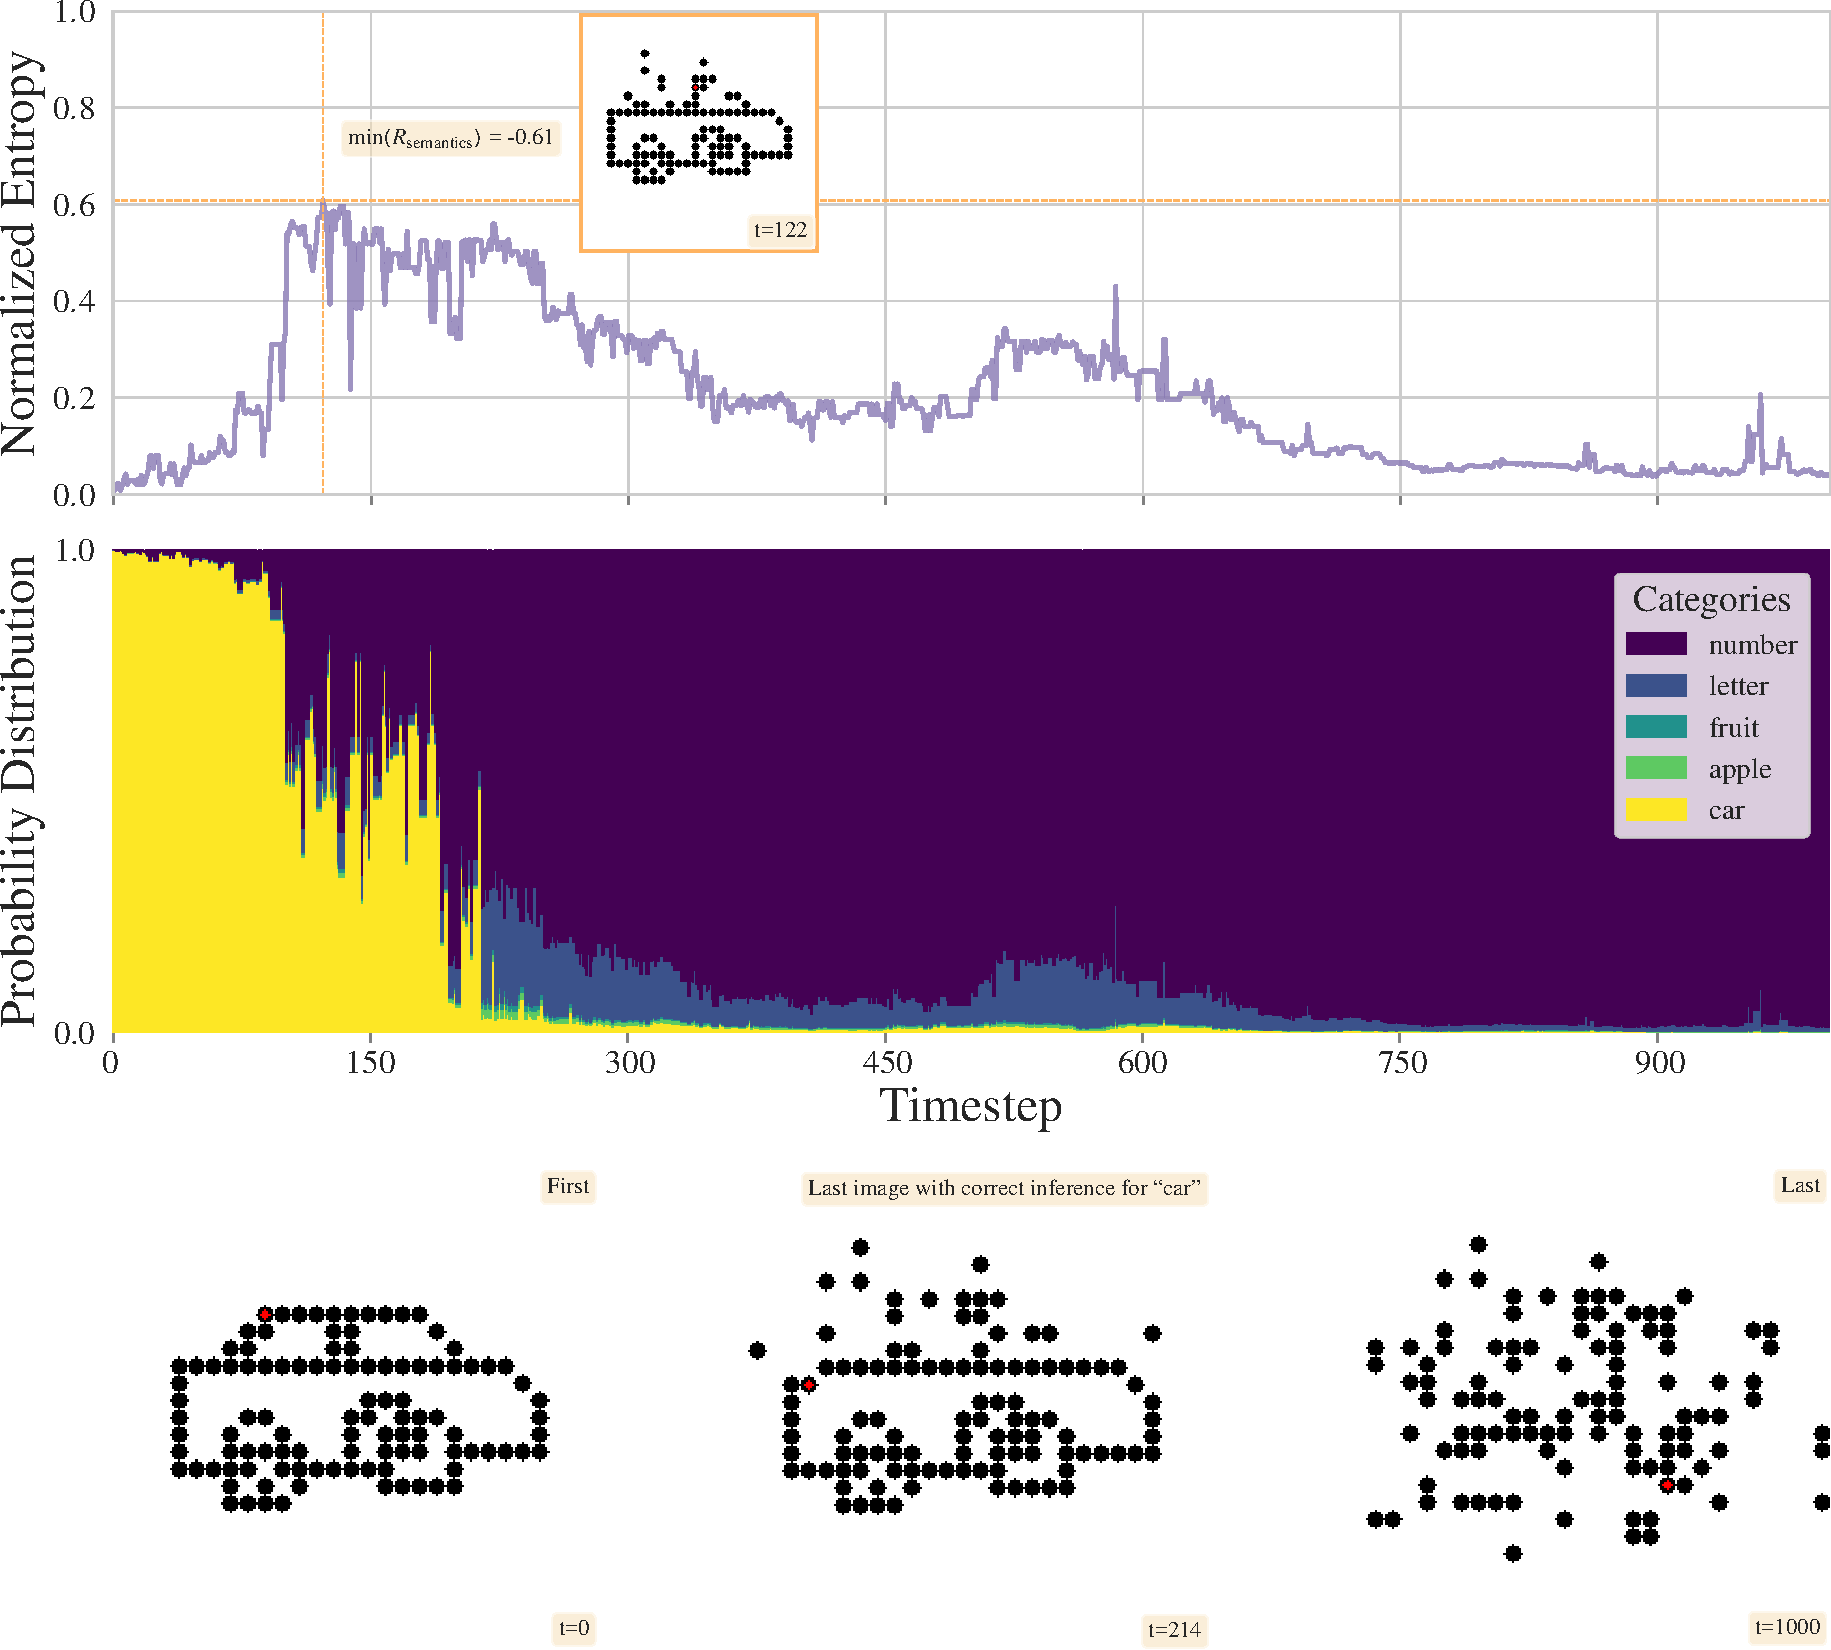
\includegraphics[width=0.8\textwidth]{images/sparse_rewards.pdf}
    \caption[Random rollouts in ShapeGridWorld.]{Random rollouts in ShapeGridWorld. Going from left to right in time, we perturb the grid pixel-by-pixel and observe CLIP's confidence change. The top row shows the distribution of CLIP's inferences over the labels ``giraffe'', ``number'', and ``random'' in red, green, and blue respectively. The first and last images in the bottom row are the initial and final images respectively.
    The middle three images in the bottom row show the images where the distribution changed its trend, at the last time when ``giraffe'' was the most confident category, at the time when the distribution was equally split between the categories, and the first time when ``random'' was the confident category.
    They are all just a few pixels away from each other but essentially still the same, yet they are much different for CLIP.}
    \label{fig:sparse-rewards}
    
\end{figure}

Sparse rewards are a problem in reinforcement learning in general because underly a lack of continuous feedback. 
With only sporadic rewards, it becomes exceedingly difficult for an agent to gauge the values of actions to lead it to eventual rewards, i.e. credit assignment becomes difficult, which in turn leads to difficult and inefficient learning of action policies.

% If we imagine this scenario in reverse with an active controller, i.e. if the agent starts from the random image and tries to converge to a meaningful image by relying on the semantics entropy reward, it might register a sudden burst of rewards for small changes in the image, but these rewards are just artifacts of the noise in CLIP's inferences.

Thus, a smooth and continuous reward is essential for effective learning.
Since we used the iCEM controller which is a gradient-free optimization algorithm and has proved to work well in sparse reward settings, it helped to mitigate this problem.

\subsection{Semantic Bias in Random Images} % Confidence in random images
\label{sec:inference-noise}
The other consequence of the noise in CLIP inference is that can sometimes confidently classify random images to a class, i.e. false positives, instead of having a flat distribution.
\figref{fig:semantic-bias-random} shows some examples of Tangram creations in which CLIP displayed high confidence.

\begin{figure}[h]
    \centering
    % \includegraphics[width=0.6\textwidth]{images/p_random_semantic_bias.png}
    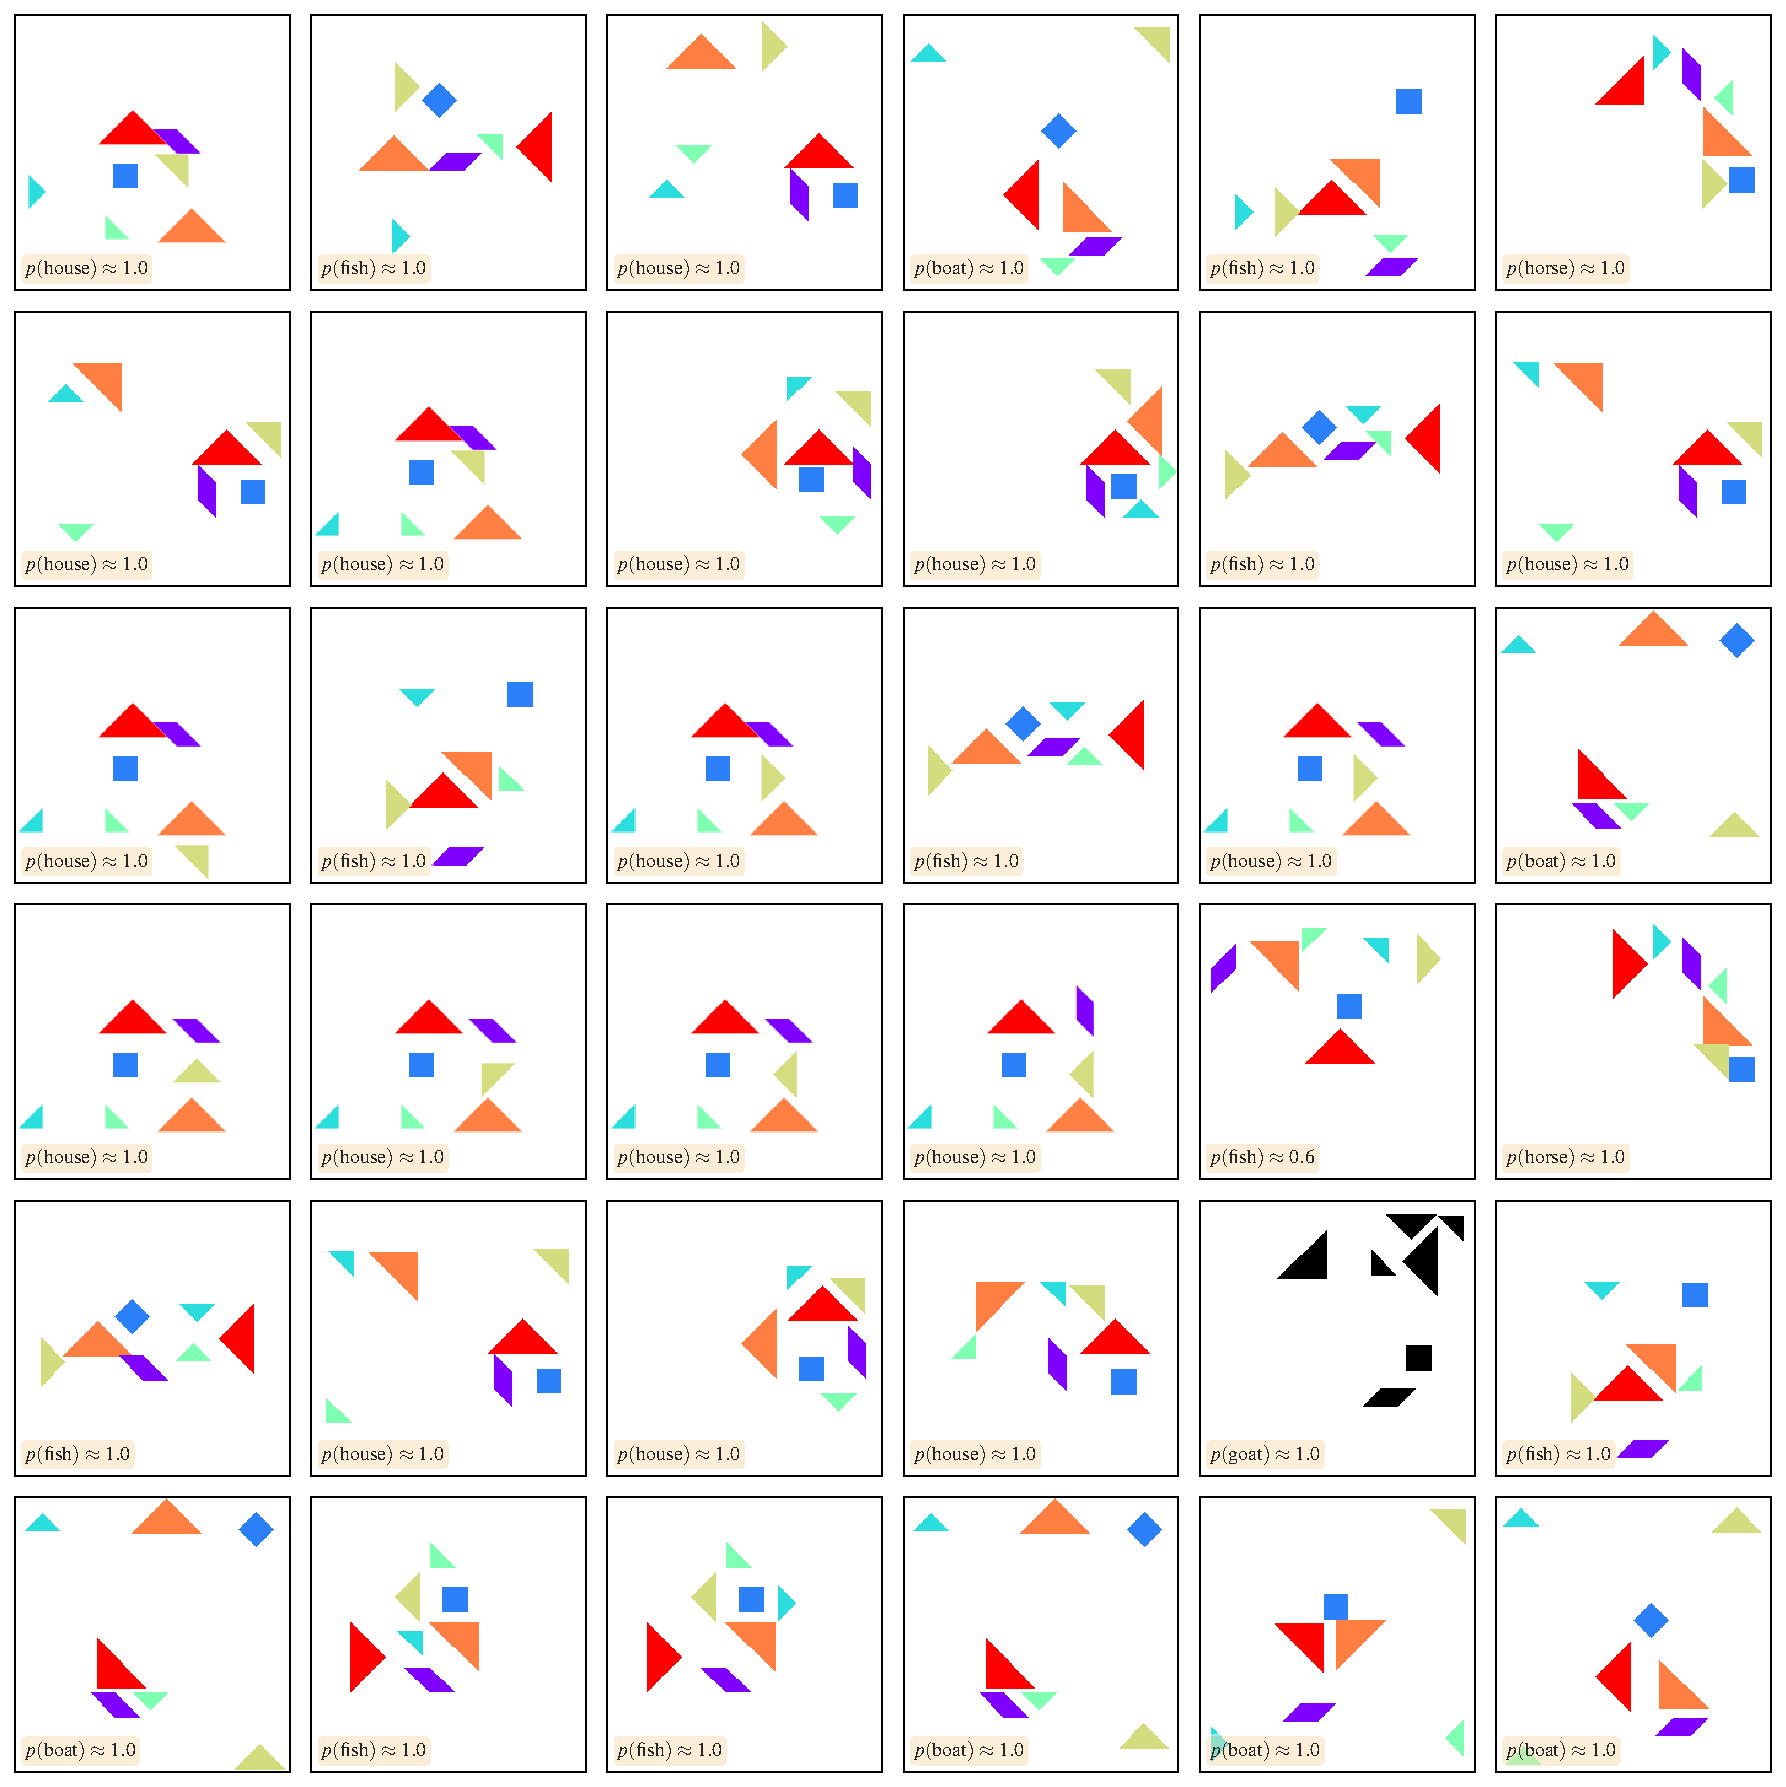
\includegraphics[width=\textwidth]{images/adversarial_samples.pdf}
    \caption{Large semantic bias in random images.}
    \label{fig:semantic-bias-random}
\end{figure}

This can also be interpreted as a jagged reward landscape with many local optima.
This noisy reward signal can lead the agent to be stuck in local optima (with a rather meaningless creation that it erroneously finds confident), or inhibit it from reaching a good optimum.

The two problems, sparse rewards and semantic bias in random images are not independent.
They have the same underlying cause -- noisy CLIP inference, yet there's a non-trivial anticorrelation between reward sparseness and noise.
That is, increasing reward density involves increasing confidence in imperfect/partial creations which also increases noise.


\subsubsection{Class Preference in CLIP}
\label{sec:class-preference}
Another complementary issue we faced related to the problem of semantic bias in random images was that of class imbalance.
Simply put, there were some classes in which CLIP was consistently more confident than others and leaned towards them over others when unsure.
This included classes that signified broad concepts like ``animal'', ``fruit'', ``number'', ``letter'', or ``object''.

% \begin{figure}[H]
%     \centering
%     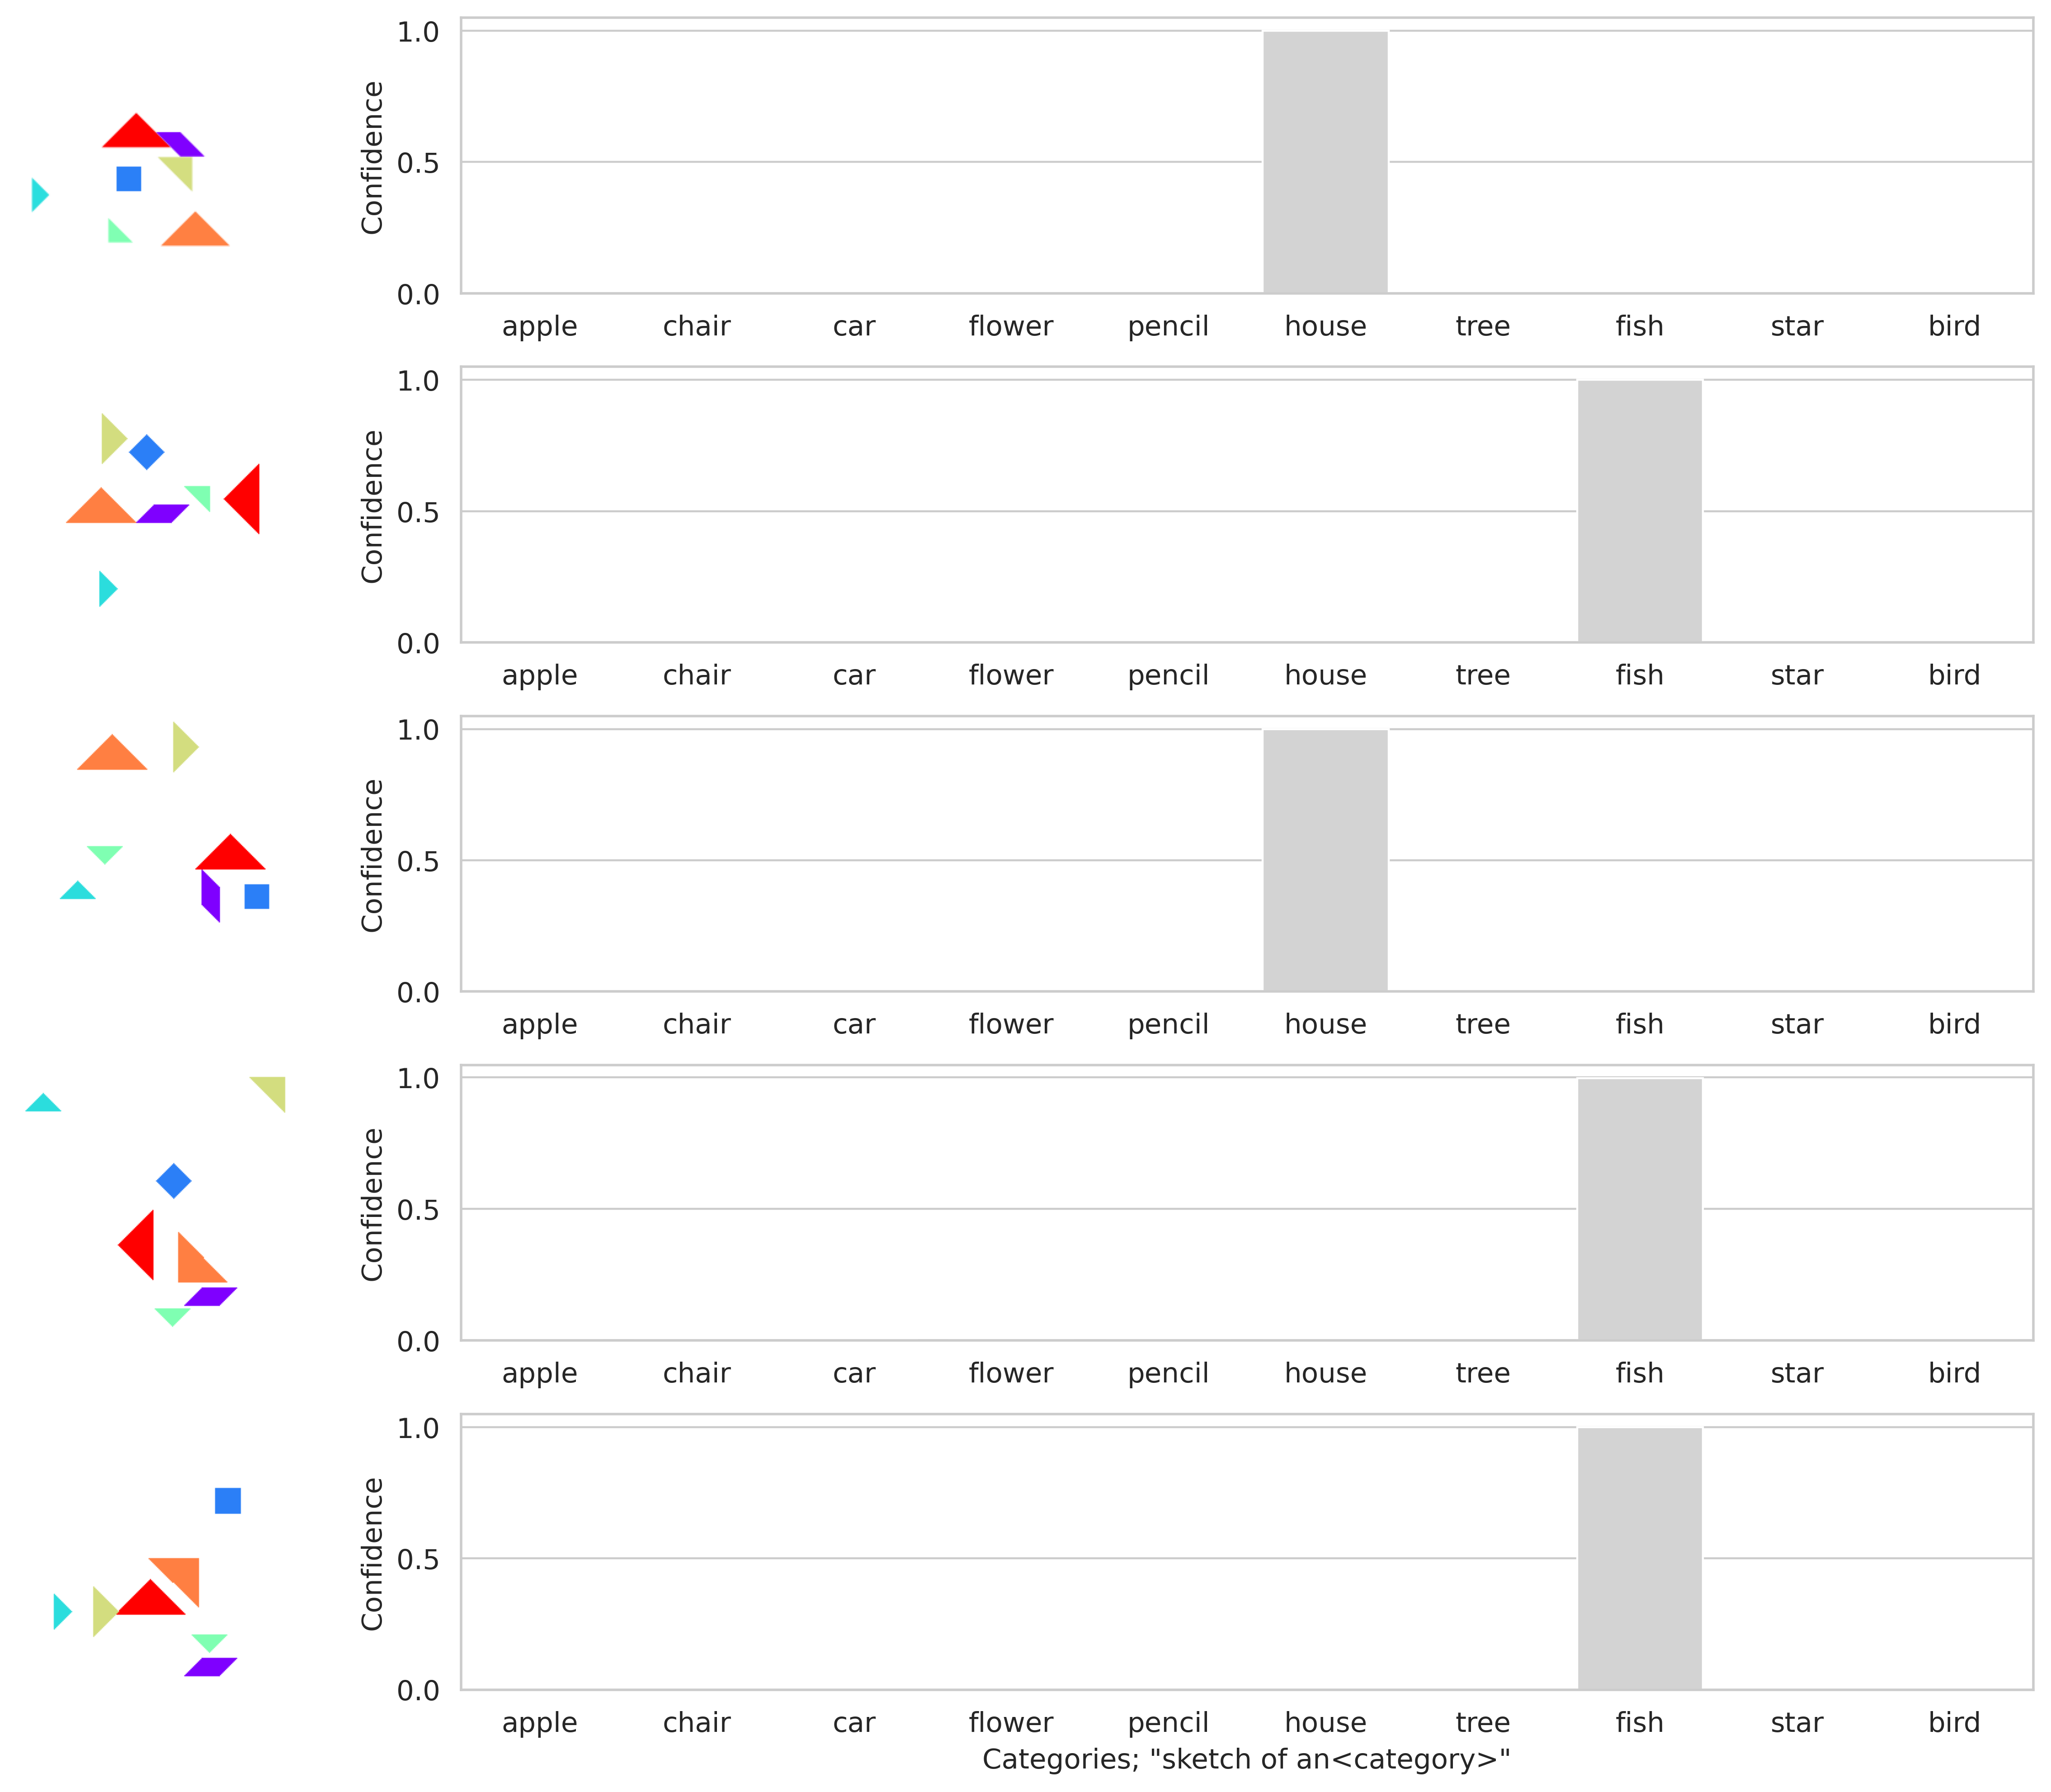
\includegraphics[width=\textwidth]{images/inference_noise.png}
%     \caption{Class preference in CLIP.}
%     \label{fig:class-preference}
% \end{figure}

This is a fundamental nature of the CLIP model and we could only mitigate it by avoiding certain categories and choosing enough categories for the semantics entropy reward such that CLIP's preferences balanced out.
More discussion on tackling this problem in particular is given in section \secref{sec:clip-categories}.

\newpage
\section{Trajectory Analysis with Closeness Costs}
\label{sec:closeness-rollouts}
% closeness_reward_scale
% closeness_reward_threshold
Before we started improving and running simulations using inferences from CLIP, we needed to ensure that the controller was able to reach a reward-conditioned goal in our environments, i.e. it was \emph{solvable}.
Especially, it was crucial to establish this solvability under sparse rewards.

To ensure that our controller did this efficiently and robustly, a good choice of the iCEM controller hyperparameters and the environment configuration was essential.
These hyperparameters and configurations were dependent on each other so we needed to optimize them together.

For example, for both environments, the size of the grid together with the step size affects the minimum required planning horizon for the controller.
For a small discrete grid or a large enough step size, the planning horizon does not need to be very high, because the controller can potentially reach the goal in a few steps and does not need to plan far ahead.
If the step size is too small for the grid size, a longer planning horizon is required so that the agent can discover the reward by random sampling.

In a similar vein, the step size is also related to the \emph{object persistency} used in the environments.
This parameter governs how many steps a single object (pixel block in ShapeGridWorld and a polygon in Tangram) is in focus for the actions of the controller before it cycles to the next object in the sequence.
For a high object persistency, the step size could be lower, but for a low object persistency, the step size needs to be higher.

These interdependencies made the hyperparameter optimization problem quite complex and the sheer number of these parameters made this task very expensive.
Given the high computation resources and time required to run simulations with the semantics entropy reward using CLIP, it was infeasible to do a proper search over all the hyperparameters.
Thus, we instead used an alternative reward function to analyze the effect of the hyperparameters.
We called this ersatz reward function the \emph{closeness reward}.

A closeness reward is defined in the context of a fixed target creation in the environment, and its function is given as the negative of a distance function between the current creation and the target creation in the state space of the environment.

We used two different formulations of the distance function, which we called the \emph{dense closeness cost} and \emph{sparse incremental closeness cost}.
The dense closeness cost is formulated as the \(L^2\) distance between the current and target creations and the sparse incremental closeness cost is formulated as the dimension-wise thresholded \(L^1\) distance between the current and target creations, given by,
\begin{equation}
    \label{eq:closeness-reward-sparse}
    d(\bfi, \bft) = \sum_{k \in n_s} \bm{1}_\varepsilon(\bfi_k - \bft_k),
\end{equation}
where \(\bfi, \bft \in \cS\) are the current and target creations respectively, \(\varepsilon\) is a small threshold, and \(\bm{1}_\varepsilon\) is the indicator function such that \(\bm{1}_\varepsilon(x) = 1\) if \(|x| > \varepsilon\) and \(0\) otherwise.

\todo{add more details about the hyperparameters optimized here.}

Using the closeness reward/cost formulations, we performed an extensive grid search over the many hyperparameters of the iCEM controller and the environment together to find the best combinations and study their effects.
To assess and compare the results in these experiments, we compared their cumulative rewards over the rollouts.

The controller was easily able to achieve the goal under dense closeness rewards for a wide range of hyperparameters and other than a few parameters such as the granularity of the grid, the step size, and the object persistency, we did not notice much difference in the performance of the controller over the other hyperparameters.
\figref{fig:closeness-rollouts} shows a sample closeness reward run for the dense closeness cost on the Tangram environment.

The tuning was more difficult under sparse incremental rewards, which required a higher planning horizon and more sampled trajectories to reach the goal.
This directly corresponds to a higher computational cost.

The cost aggregation functions \texttt{best} and \texttt{sum} were comparable in performance and performed better than \texttt{best-\emph{l}}, \emph{last}, and \emph{last-\emph{l}}.
We typically employed the \texttt{sum} aggregation function as it is more robust to noise due to its summation.
In other runs, we found the greedier \texttt{best} aggregation function to be more efficient in reaching the goal and escaping local minima.

The comparison results are omitted here for brevity. Please refer to the appendix sections \ref{sec:icem-details} and \ref{sec:environments-details} for more details about these hyperparameters of the iCEM controller and the environments respectively.

From this analysis, we were able to gain an intuition of the minimal required set of hyperparameters that allowed the controller to solve the environment.
These minimal parameters were then used as a starting point for the simulations with the semantics entropy reward.

\begin{figure}[H]
    \centering
    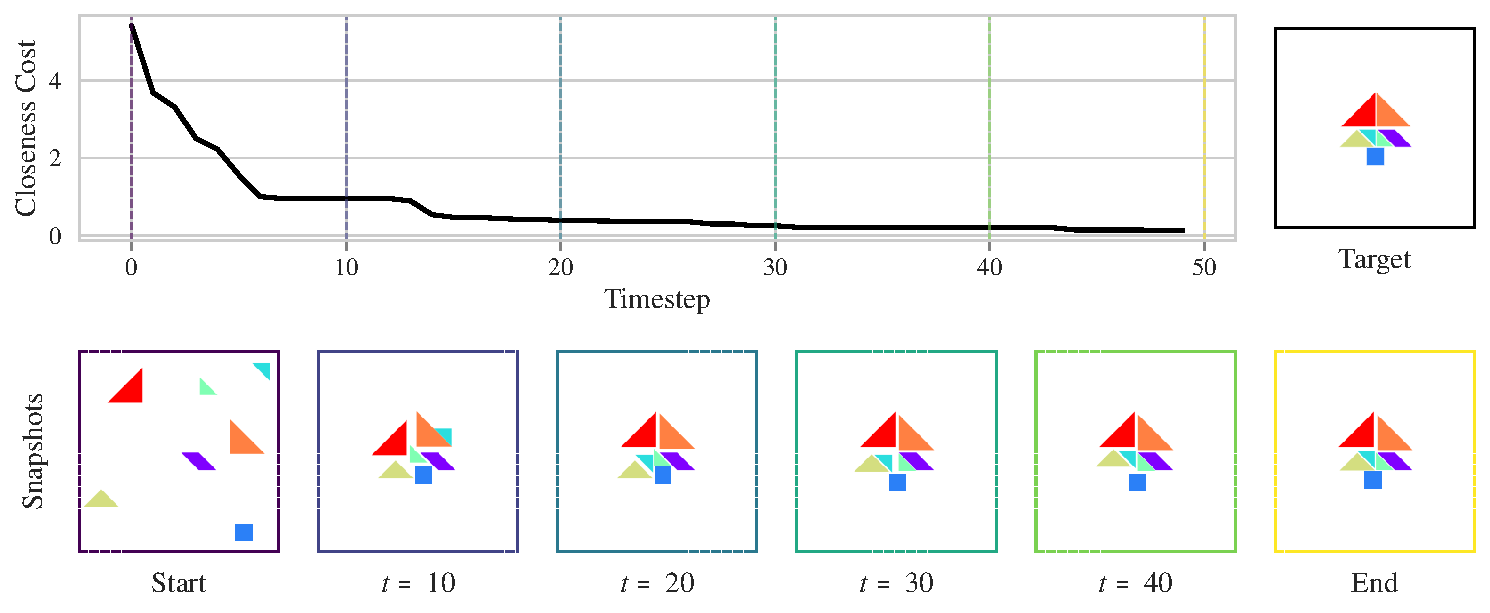
\includegraphics[width=\textwidth]{images/closeness_trajectory_495.pdf}
    \caption{A successful closeness cost rollout in Tangram.}
    \label{fig:closeness-rollouts}
\end{figure}


% \subsubsection{Tuning Environment Parameters}
% \label{sec:env-hyperparameters}
% % render_kwargs.invert
% % render_kwargs.color

% \label{sec:sgw-hyperparameters}
% % width
% % x_step
% % render_delta
% % object_persistency
% % max_dist
% % control
% % control_boundaries


% \label{sec:tangram-hyperparameters}
% % flip
% % rotate
% % x_size
% % r_size
% % x_step
% % object_persistency
% % max_dist
% % control
% % control_boundaries
% % staging_boundaries


% \subsubsection{Tuning Controller Hyperparameters}
% \label{sec:icem-hyperparameters}
% % action_sampler_params.opt_iterations
% % action_sampler_params.init_std
% % action_sampler_params.elites_size
% % num_simulated_trajectories
% % horizon
% % cost_along_trajectory
% % discount_along_trajectory

% \todo{Talk about the different hyperparameters that were considered. Show histograms of only the significant parameters.}

\newpage
\section{Improving CLIP Rewards}
\label{sec:improving-rewards}

We experimented with several methods to reduce the noise from CLIP.
The regularized semantics reward also has many hyperparameters that can be tuned to make the reward landscape smoother.
Namely, the temperature of the softmax function (\(T\)), the target baseline regularization strength (\(\alpha\)), the image baseline regularization strength (\(\beta\)), the use of negative embeddings, and tweaking the rendering function (adding texturing or modifying the images with other operations).

The complex nature of the reward landscape and the high dimensionality of the state space made it difficult to analyze the effects of these hyperparameters.
To gain an intuition over these parameters and reduce the search space before we ran simulations using them in the full semantics reward, we instead used the best of the previously rolled-out trajectories with the closeness reward from \secref{sec:closeness-rollouts} and ran post hoc inference on the resulting sequence of image observations using CLIP and calculated the trajectories of the resulting semantics reward\footnote{The myriad of combinations due to the high dimensional space makes it infeasible to show all the subtleties of the interplay between these hyperparameters in a few figures.
Thus, we have additionally made the analysis available for the reader as an interactive notebook at \url{https://colab.research.google.com/drive/1UzKb5t5PDRO05GbSKpgzWd3DELfAzDxJ} or \url{https://t.ly/j84on}, where one can pick a combination of different hyperparameters, and prefixes and suffix to see their effects}.

The performance (cumulative rewards) can highly depend on the choice of prefix and suffix (\figref{fig:prefix-suffix}).
\begin{figure}[h]
    \centering
    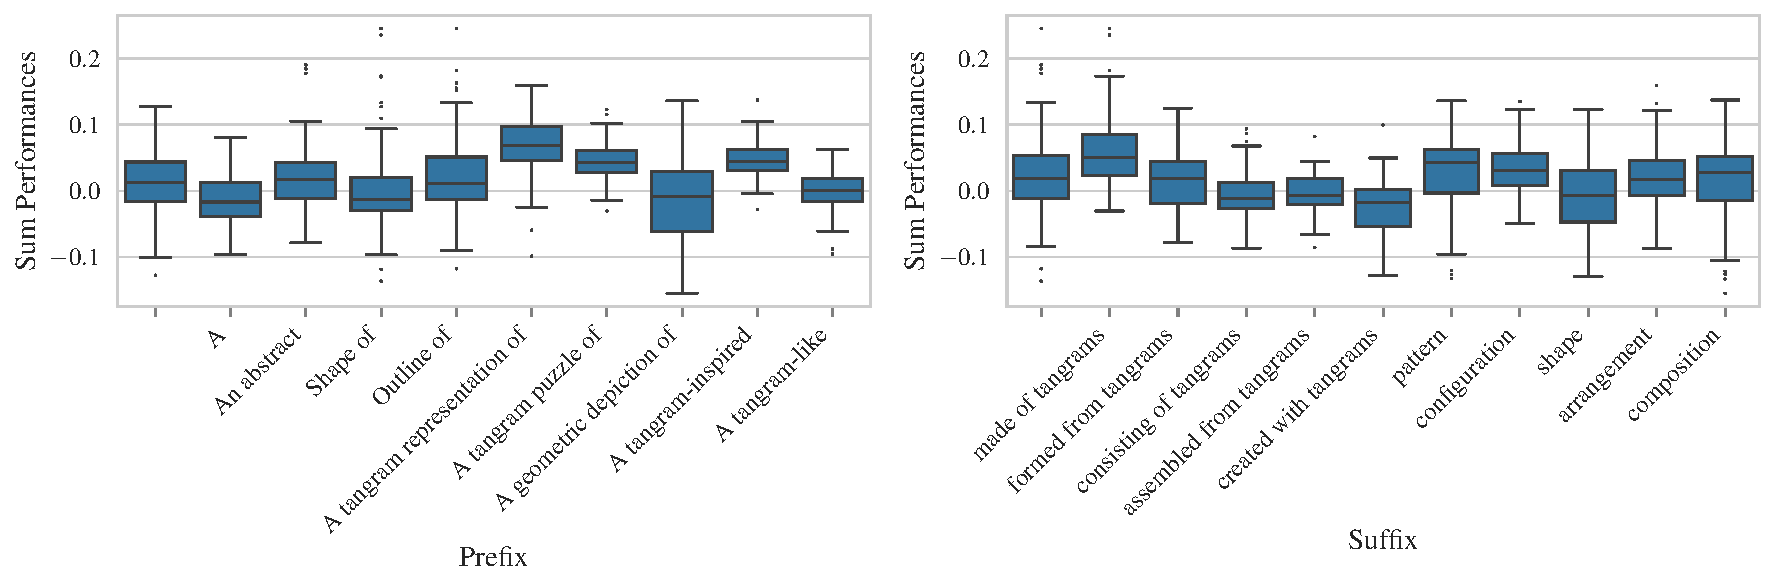
\includegraphics[width=\textwidth]{images/prefix-suffix.pdf}
    \caption{Effect of different prefixes and suffixes on semantics entropy reward trajectories.}
    \label{fig:prefix-suffix}
\end{figure}

To get the underlying trends in these parameters and find robust values that are agnostic to prompt engineering, i.e. the choice of prefix and suffix in formulating the text input, we average over our results across multiple choices and combinations of these text prefix-suffix pairs.

We observed clear trends in the effects of these hyperparameters on the reward landscape.
Consequently, we performed an ablation study on these hyperparameters independently to gain insights into their effects.
The following sections on the specific hyperparameters discuss the results of these analyses.
In the figures shown in these sections, we choose the best-performing other hyperparameters.
These results can be compared to the corresponding adversarial study results discussed in \secref{sec:adversarial-performance}.

\subsection{Effect of the Number of Creative Possibilities}
\label{sec:clip-categories}
To alleviate the problem of class preference in CLIP, we experimented with different numbers of categories/creative possibilities (\(c\)) for the semantics entropy reward.
\figref{fig:clip-categories} shows the effect of the number of categories on the entropy of CLIP inferences over a random image.

\begin{figure}[H]
    \centering
    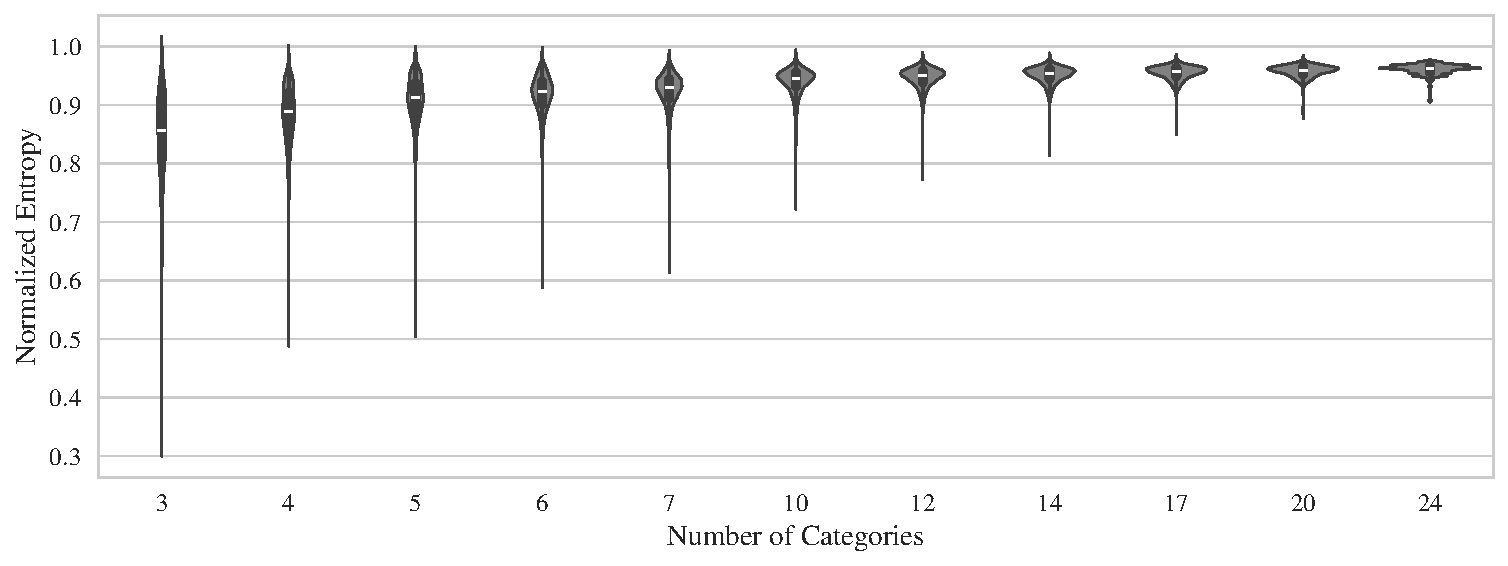
\includegraphics[width=\textwidth]{images/category_comparison_tangram.pdf}
    \caption{Effect of the number of categories on CLIP inference distribution over a random image.}
    \label{fig:clip-categories}
\end{figure}

We observed that too few categories can promote semantic bias and class preference in random images, but too many categories can exacerbate the problem of noisy rewards since there are potentially more misleading distractions for the agent.

It was important to choose categories that were semantically distinct and not too broad which was non-trivial.
Especially for the Tangram environment, in which the creations can be quite abstract, there was only a limited set of feasible categories.
This suggested that a moderate number of categories would be optimal.
For our simulations, we typically chose a set of \(10 \sim 20\) categories.

\subsection{Effect of Temperature}
\label{sec:reg-temperature}
% semantics_model_temperature

Temperature is a crucial hyperparameter for the softmax function in the semantics entropy reward as it directly controller the entropy of the CLIP distribution.
The original CLIP publication recommends a temperature of \(0.01\) for most use cases, which we also found to most often work best.
Temperatures up to \(0.02\) were good as well.
Any temperature below this range performed significantly worse as it exacerbated the noise of CLIP, and any temperature above this range made the reward landscape too smooth and the reward trajectories too flat.

\figref{fig:clip-temperature} shows the effect of temperature on the semantics entropy reward trajectories, averaged over multiple choice of categories.
This is a post hoc CLIP inference on trajectory samples from the closeness reward rollout experiments.

\begin{figure}[H]
    \centering
    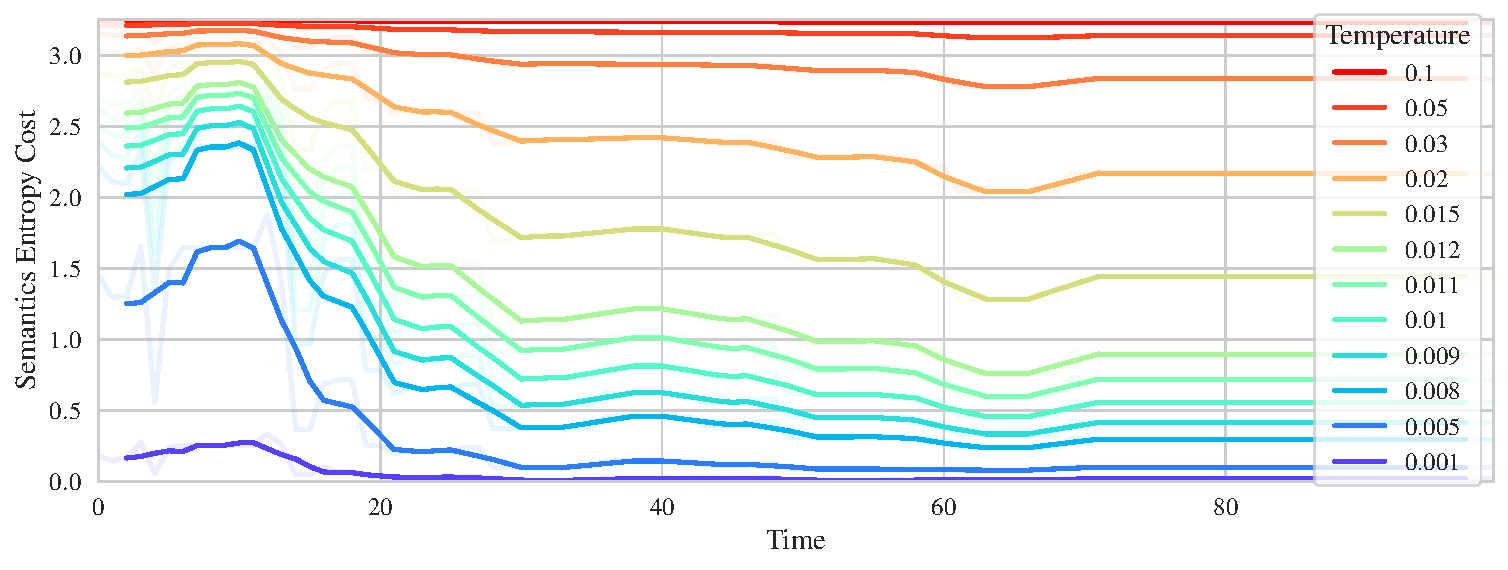
\includegraphics[width=\textwidth]{images/temperature_comparison.pdf}
    \caption{Effect of temperature on semantics entropy reward trajectories.}
    \label{fig:clip-temperature}    
\end{figure}

\subsection{Effect of Baseline Regularization}
\label{sec:reg-alpha-beta}
% semantics_alpha_target

The regularization strength of the target baseline (\(\alpha\)) and the image baseline (\(\beta\)) were arguably the most important hyperparameters for the regularized semantics entropy reward.
Baseline regularization helps with the problem of sparse rewards by providing better directional guidance in the CLIP embedding space.

The motivating study of \emph{VLM-RM} noted the best value of the target baseline regularization strength in goal-regularized settings to be somewhere in the middle of the two extremes.
We found a similar trend in our experiments, with a slight preference for the additional image baseline regularization strength to be higher than the text baseline regularization strength.

In our analysis, we compared the cumulative rewards of the post hoc inferences on closeness reward trajectories with different values of \(\alpha\) and \(\beta\) to find the optimal values.
\figref{fig:clip-alpha-beta} shows these results, averaged over multiple choice of prefixes and suffixes.

\begin{figure}[H]
    \centering
    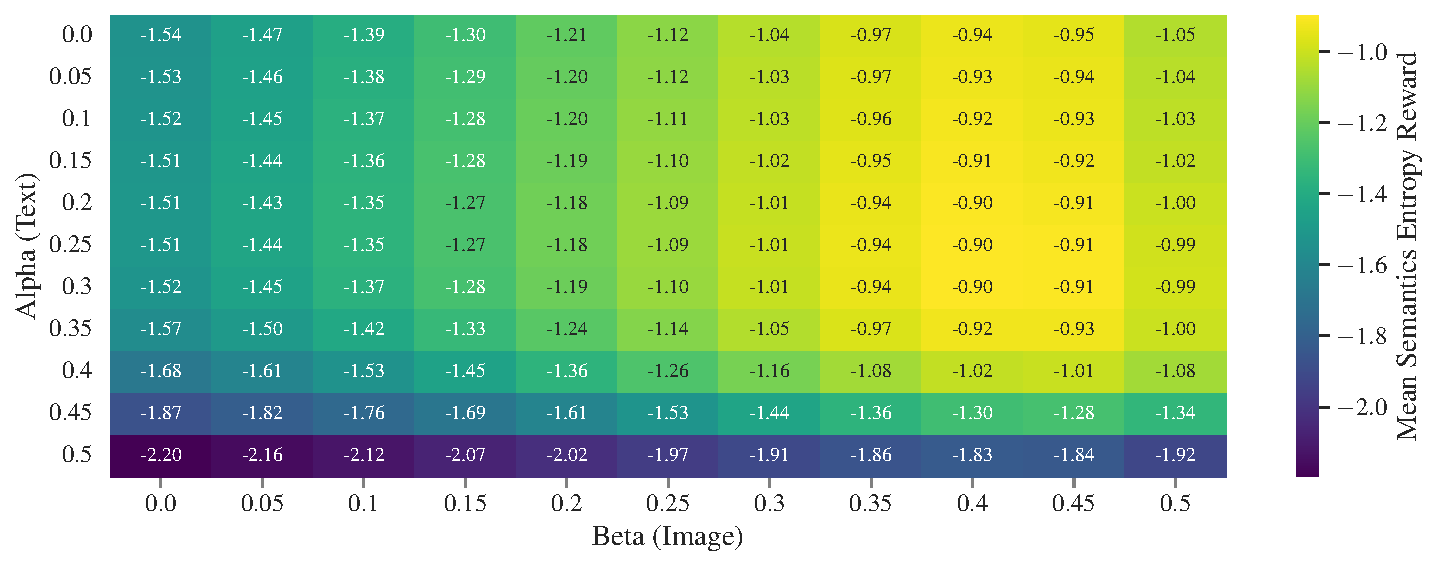
\includegraphics[width=\textwidth]{images/alpha_beta_temp12avg_noneg.pdf}
    \caption{Effect of regularization strength on semantics entropy reward trajectories.}
    \label{fig:clip-alpha-beta}
\end{figure}


% \subsection{Effect of Changing Prefix and Suffix}
% \label{sec:prefix-suffix}
% % label_prefix
% % label_suffix
% Different prefixes/suffixes and combinations of them also affected the performance of CLIP.

% \begin{figure}[H]
%     \centering
%     \missingfigure{Effect of changing the prefix suffix.}
%     \caption{Effect of different prefixes and suffixes.}
%     \label{fig:prefix-suffix}
% \end{figure}

\subsection{Effect of Negative Embeddings}
\label{sec:negative-embeddings}
\cite{negprompt} used negative embeddings as target baselines in their goal-conditioned CLIP reward function to make the reward landscape smoother.
We experimented with this as well, and instead of using the initial description of the environment as the text baseline, we used a negative embedding of the target creation.

We did not find this to be helpful in our experiments, instead it seemed to flatten the reward landscape.
We think this is a consequence of CLIP's language encoder being a bag-of-words model, and the negative embeddings being essentially close to the target embeddings, which effectively zeros out the target embeddings.

\begin{figure}[h]
    \centering
    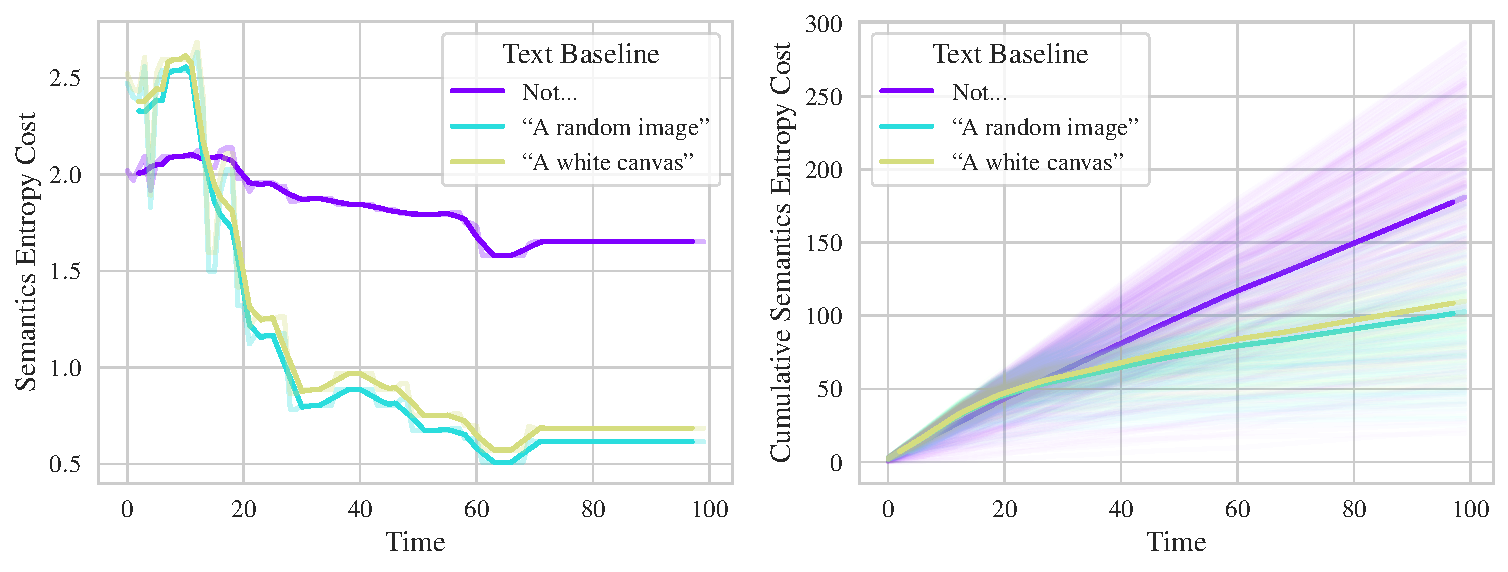
\includegraphics[width=\textwidth]{images/baseline_comparison.pdf}
    \caption{Effect of different text baselines on semantics entropy reward trajectories.}
    \label{fig:baseline}
\end{figure}

\subsection{Effect of Adding Post-Suffix}
\label{sec:post-suffix}
\cite{waffleclip} found that adding a \emph{post-}suffix to the label in the text input to CLIP improved the quality of the inferences.
This post-suffix can surprisingly even be a random string of characters.

Following these insights, we also experimented with adding a random string of jibberish to the end of the label as a post-suffix, but we did not find it to affect the reward.
\figref{fig:post-suffix} shows the effect of different post-suffixes on the semantics entropy reward trajectories, averaged over combinations of prefixes and suffixes.

\begin{figure}[H]
    \centering
    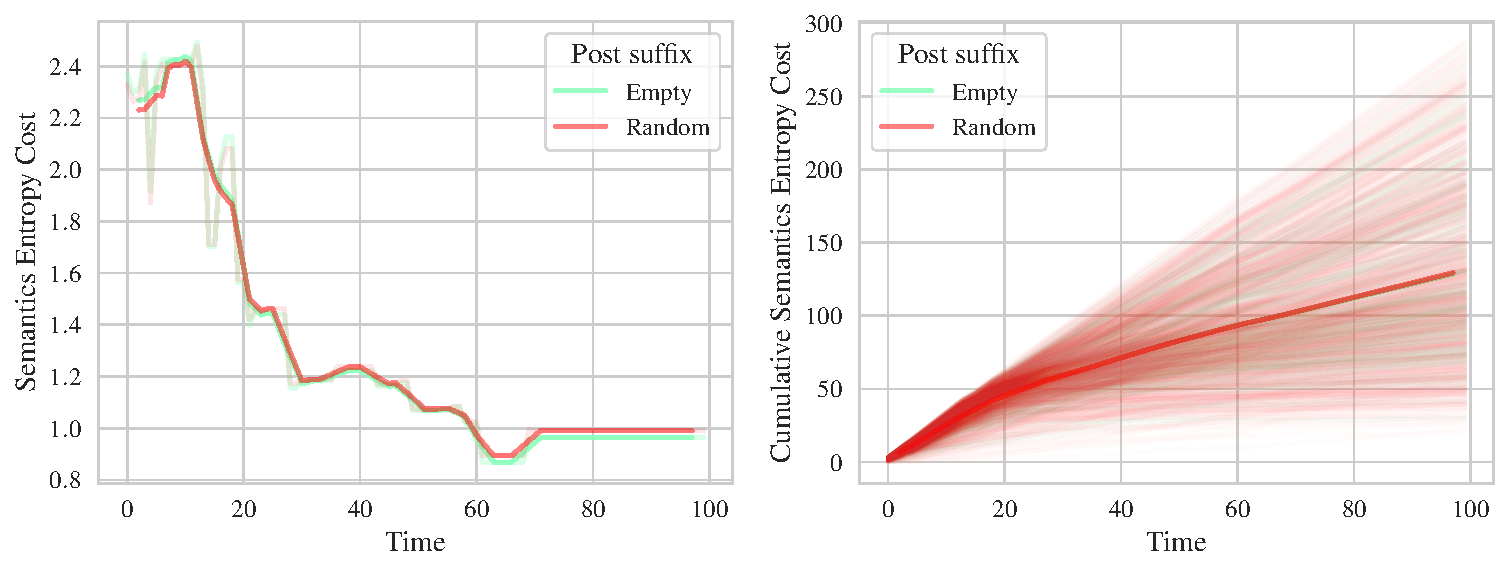
\includegraphics[width=\textwidth]{images/post_suffix_comparison.pdf}
    \caption{Effect of different post-suffixes on semantics entropy reward trajectories.}
    \label{fig:post-suffix}
\end{figure}

% \begin{figure}[H]
%     \centering
%     \missingfigure{As a consolidation of everything before, a bar plot with ablations.}
%     \caption{Ablations of the different methods to improve semantics entropy reward.}
%     \label{fig:clip-ablation}
% \end{figure}

% \newpage
\subsection{Entropy Regularization}
\label{sec:entropy-regularization}
Another promising way to make the reward landscape of CLIP smoother is to fine-tune it with an additional entropy regularization loss over its output.
This is given by,
\begin{equation}
    \label{eq:entropy-regularization}
    L(\bmi, \bml) = L_{\iota}(\bmi, \bml) \underbrace{+ \kappa \sum_{\bfi_k \in \bmi}\sum_{\bfl_j \in \bml} p(\bfl_j; \bfi_k, \bml) \log p(\bfl_j; \bfi_k, \bml)}_{\text{Entropy Regularization}},\\
\end{equation}
where \(L_{\iota}\) is the contrastive cosine-similarity loss used to train CLIP, $\kappa$ is the regularization strength, and \(p(\bfi_k, \bml)\) is the classification probability distribution of image \(\bfi_k\) over the labels \(\bml\) predicted by CLIP.

We experimented with this regularization method to train a toy convolutional neural network (CNN) for classifying handwritten digits from the MNIST dataset \citep{mnist}, which we called \emph{Flatnet}.
Additionally, we used this in tandem with an augmented training dataset with varying sizes of random-image samples labeled with a uniform distribution over the categories.

This was quite effective in reducing the noise of the model; it seemed to relieve both of the problems from \secref{sec:clip-problems} -- the reward trajectory was smoother, and we observed less semantic bias in random images and even less class preference for random inputs.

Yet, we did not use it to fine-tune CLIP to constrain the scope of the project given the limited time.
More information on this analysis can be found in appendix \ref{sec:flatnet}.

% \newpage
\subsection{Adversarial Performance}
\label{sec:adversarial-performance}
To tackle the problem of semantic bias in random images, we collected samples of the false positive image observations from our rollouts, called \emph{adversarial observations} (\figref{fig:semantic-bias-random}), by filtering out the image observations with low entropy from all our runs and then manually removing the ones that were true positives.
Then, we searched for the semantics reward regularization hyperparameters that make CLIP less confident in the adversarial images while maintaining its inference for the truly semantically expressive images, i.e. increase its specificity while maintaining its sensitivity.

We used the difference in mean entropy of distributions for the false positive and true positive images as a metric to gauge the performance of CLIP.
\figref{fig:clip-temperature-adversarial} to \ref{fig:post-suffix-adversarial} show the effect of temperature, regularization, negative embeddings, and post-suffixes on discerning true positives from false positives.

\begin{figure}[H]
    \centering
    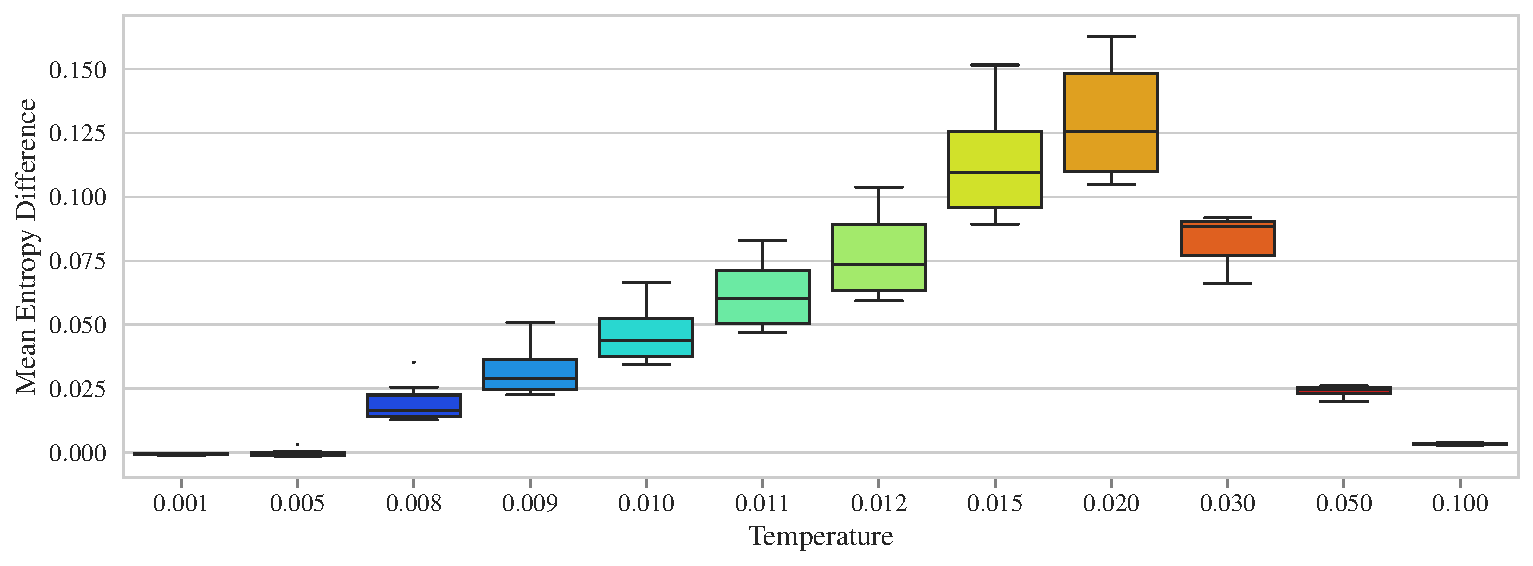
\includegraphics[width=\textwidth]{images/temperature_adversarial.pdf}
    \caption{Effect of temperature on discerning true positives from false positives.}
    \label{fig:clip-temperature-adversarial}
\end{figure}

Higher temperatures of \(2\) were better at smoothing the reward landscape just enough to improve its adversarial performance.

\begin{figure}[H]
    \centering
    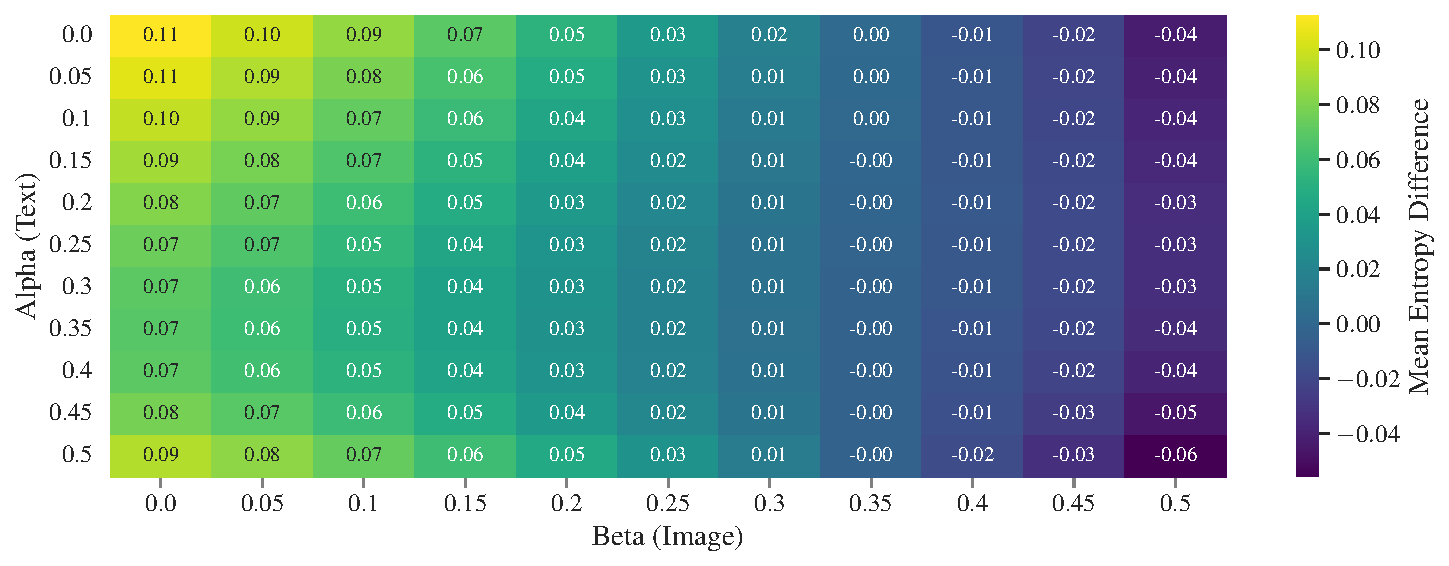
\includegraphics[width=\textwidth]{images/alpha_beta_adversarial.pdf}
    \caption{Effect of regularization strength on discerning true positives from false positives.}
    \label{fig:clip-alpha-beta-adversarial}
\end{figure}

Interestingly, the trends in the regularization strength of the text baseline (\(\alpha\)) and the image baseline (\(\beta\)) shown in \figref{fig:clip-alpha-beta-adversarial} were essentially opposite from the ones in \figref{fig:clip-alpha-beta} that showed the effect on the reward landscape.
An optimal choice of baseline strength for reducing the sparsity of the goal-based reward landscape essentially improves the path to this goal by improving the gradients to reach this desired reward.
This means that it changes the reward at near-goal status in such a way that it is better and hinting the agent if it's close to its ultimate goal, i.e. it increases the similarity or correspondance to this state to the goal state.
This is in contrast to the adversarial performance where we desire to make this difference more pronounced.
Thus, these results are not at odds with each other, but rather complementary. 

\begin{figure}[H]
    \centering
    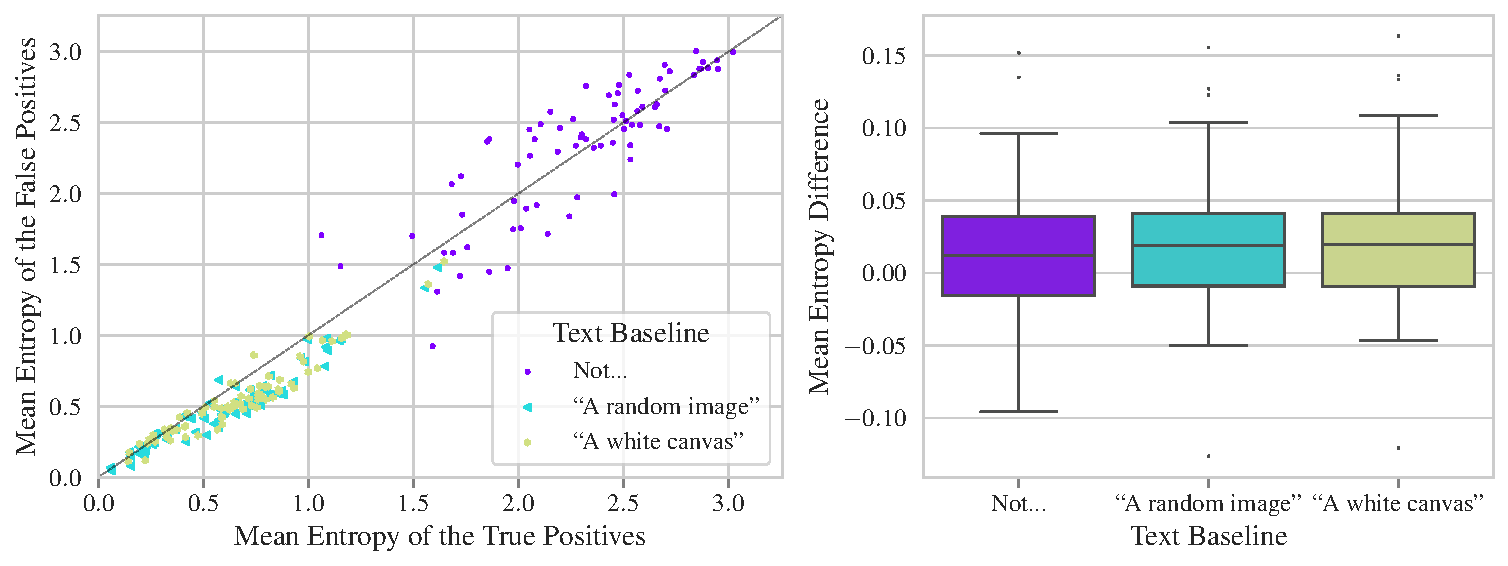
\includegraphics[width=\textwidth]{images/baseline_adversarial_2.pdf}
    \caption{Effect of different text baselines on discerning true positives from false positives.}
    \label{fig:baseline-adversarial}
\end{figure}

\figref{fig:baseline-adversarial} left subfigure shows the adversarial performance of negative embeddings in a 2D space.
Each of the points is a different combination prefix and suffix for the text input.
Ideally, we would like the points to live above the diagonal, i.e. the entropy of the false positives should be higher than the true positives.

Negative embeddings as we have seen before, flatten the reward landscape uniformly and as a consequence increase the entropy of the true positives as well.
This results in no performance improvement in the adversarial case.

\begin{figure}[H]
    \centering
    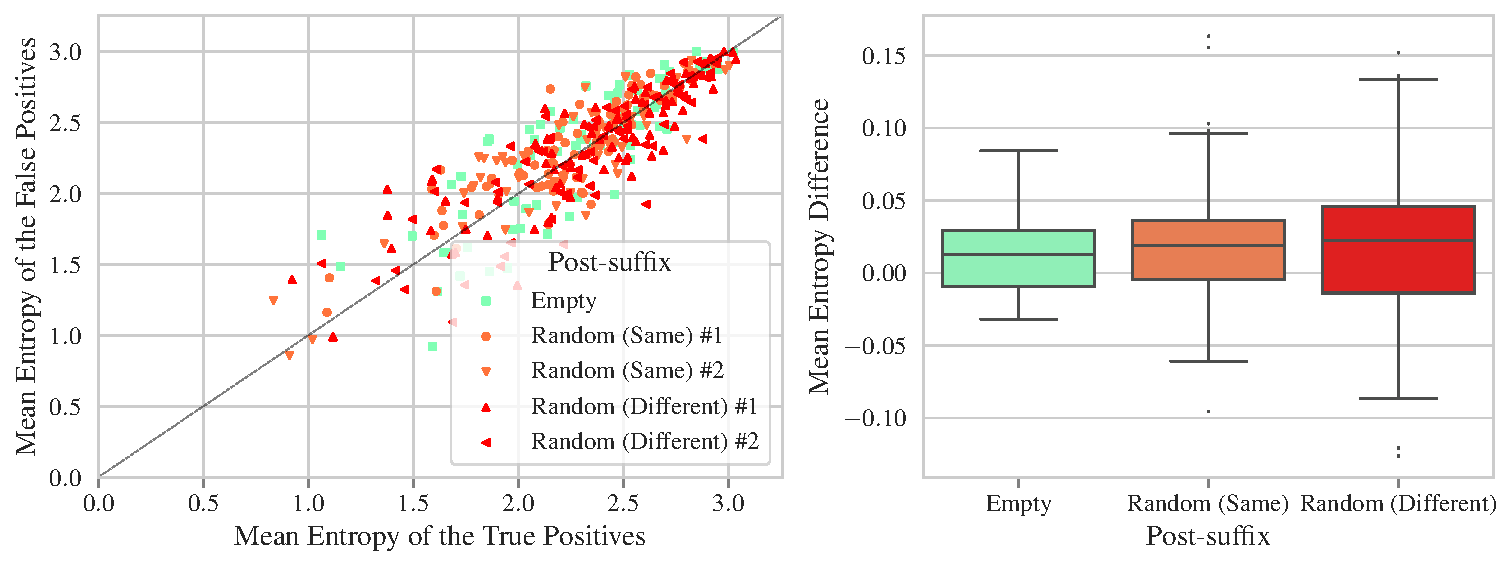
\includegraphics[width=\textwidth]{images/post-suffix_adversarial_2.pdf}
    \caption{Effect of different post-suffixes on discerning true positives from false positives.}
    \label{fig:post-suffix-adversarial}
\end{figure}

\figref{fig:post-suffix-adversarial} shows the effect of different post-suffixes on the adversarial performance.
Since we were not sure of the exact mechanism for choosing a post-suffix that would work well in general, for this analysis, to ensure more exhaustive and rigorous tests, we also used different formulations of the post-suffix and considered cases such as having the same random post-suffix across all the categories for every prefix-suffix combination or having a random one for each of the categories and combinations.
As before, we see no difference in adding or omitting the post-suffix.

% \begin{figure}[H]
%     \centering
%     \includegraphics[width=\textwidth]{images/p_subplots/rair_.pdf}
%     \includegraphics[width=\textwidth]{images/p_subplots/entropy_.pdf}
%     \includegraphics[trim=1.6cm 0cm 0cm 0cm, width=\textwidth]{images/p_subplots/distribution_.pdf}
%     \includegraphics[width=\textwidth]{images/p_subplots/snapshots_.pdf}
%     \caption{A sample rollout distribution plot.}
% \end{figure}


\subsection{Effect of Image Texturing}
\label{sec:image-texturing}
Following the observations from \cite{vlmrm}, to make the image inputs to CLIP more photorealistic to ensure in-distribution performance, we also experimented with adding textures to the images to make them more realistic for CLIP in hopes of improving its quality.
This texturing was done by adding a constant shading to the Tangram polygons.
\figref{fig:texturing-operations} show the effects of this texturing on the reward landscape.
We did not find a significant improvement in the reward landscape with this texturing.

\subsection{Effect of Image Operations}
\label{sec:image-operations}
% Shearing and Hatching
We also had the idea to use subtle image operations like shearing before inference.
We expected the true positive semantic inferences to be invariant to these operations, but the false positives to be reduced, thus reducing the noise in the reward landscape.

This is compared together with the texturing operations in \figref{fig:texturing-operations} and \figref{fig:texturing-operations-adversarial} to study their effects on the reward landscape and the adversarial performance respectively.

\begin{figure}[H]
    \centering
    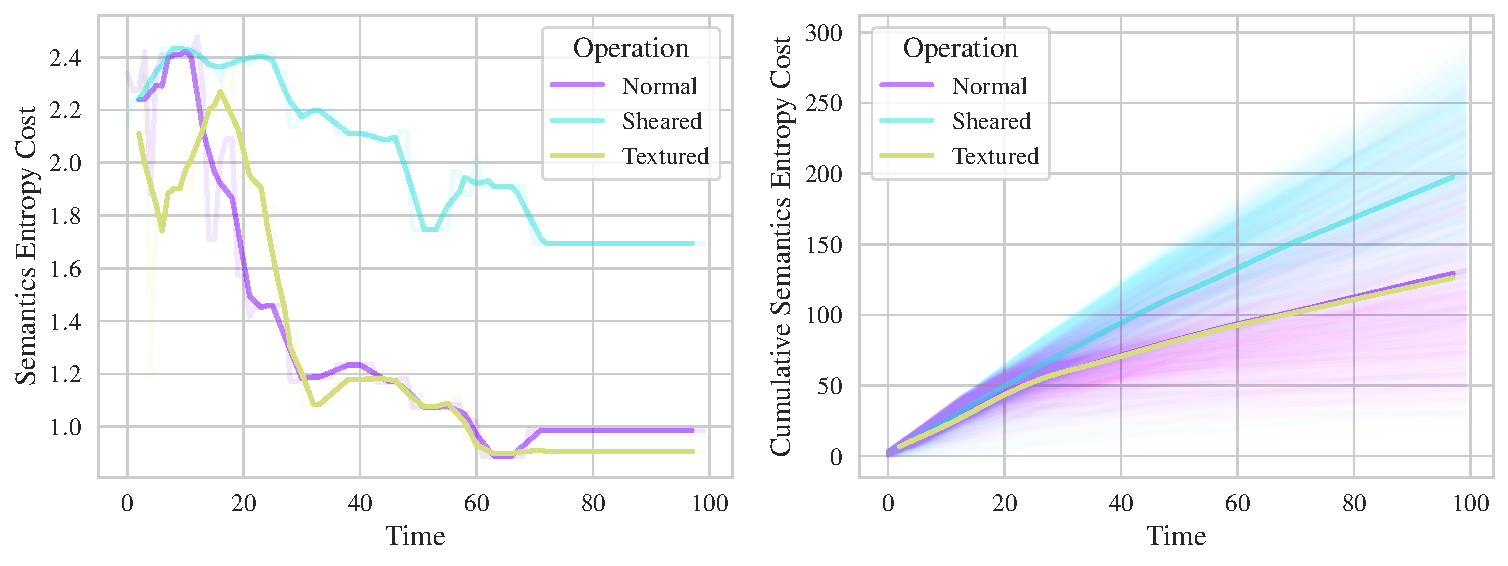
\includegraphics[width=\textwidth]{images/texturing_operations_comparison.pdf}
    \caption{Effect of texturing and image operations on semantics entropy reward trajectories.}
    \label{fig:texturing-operations}
    \vspace{12pt}
    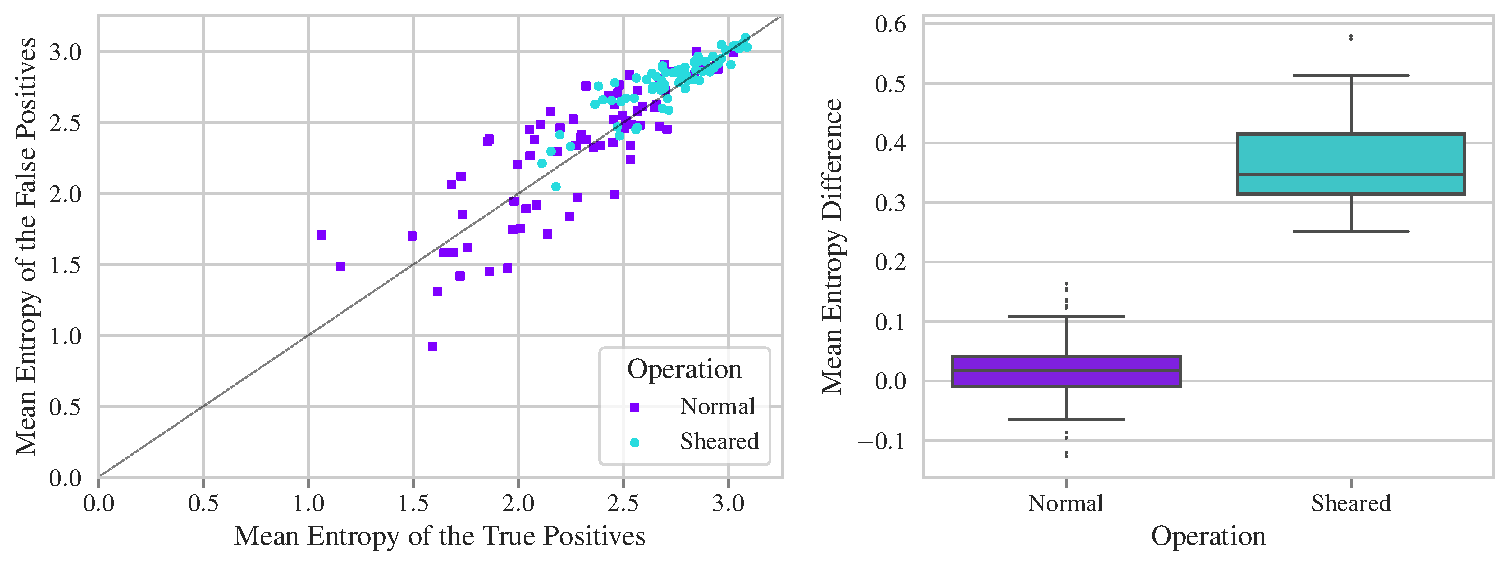
\includegraphics[width=\textwidth]{images/texturing-operations_adversarial_2.pdf}
    \caption{Effect of image operations on discerning true positives from false positives.}
    \label{fig:texturing-operations-adversarial}
\end{figure}

Shearing the images before inference did improve the quality of the inferences slightly by smoothing the reward landscape.
It had a significant performance improvement in the adversarial case as well, but it also affected the confidence in the true positive images, thus leading to lower performance by our cumulative reward metric.

To show the interdependence of the hyperparameters discussed above, \figref{fig:baseline_sheared_adversarial} and \figref{fig:post-suffix_sheared_adversarial}  compare the adversarial performance of the sheared images across negative embeddings and different post-suffix patterns respectively.
We observe that the shearing operation when used with baselines based on initial states is very helpful in improving the adversarial performance of CLIP.
Although this is helpful, in the following sections, we did not use this method, because of the associated computational costs, and because a similar effect could be achieved by tuning the regularization strengths and the temperature.

\begin{figure}[H]
    \centering
    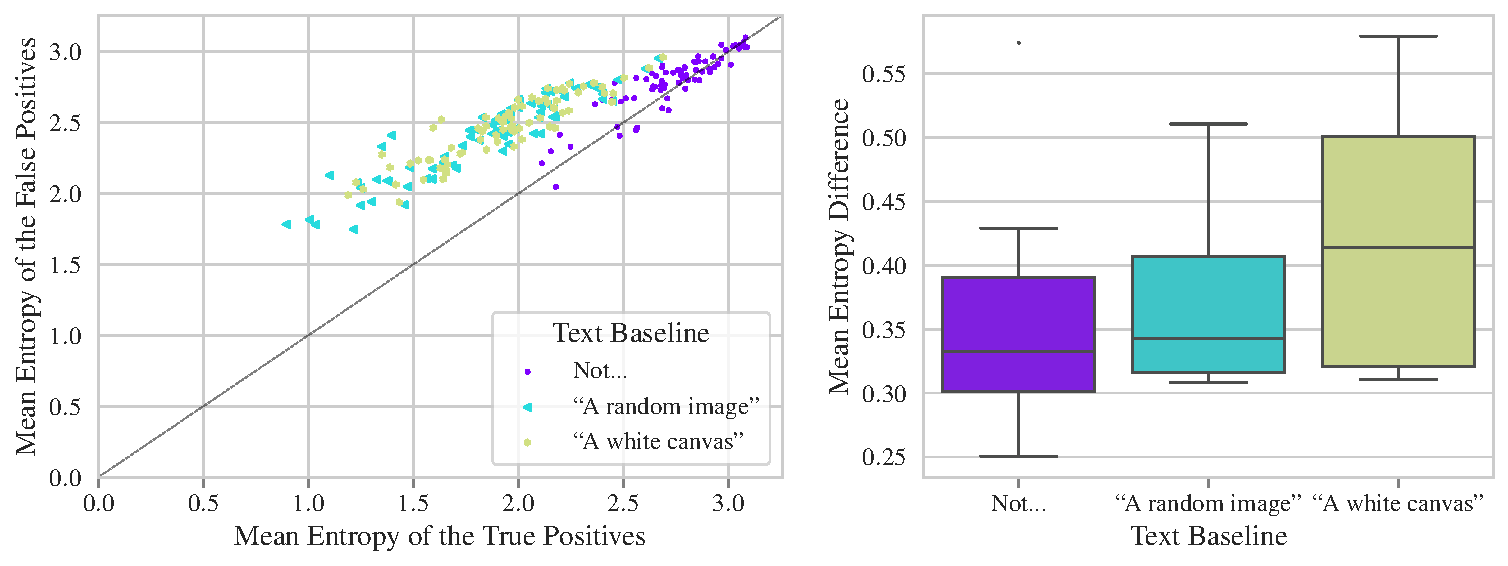
\includegraphics[width=\textwidth]{images/baseline_sheared_adversarial_2.pdf}
    \caption{Effect of different text baselines on discerning true positives from false positives with sheared images.}
    \label{fig:baseline_sheared_adversarial}
\end{figure}

\begin{figure}[H]
    \centering
    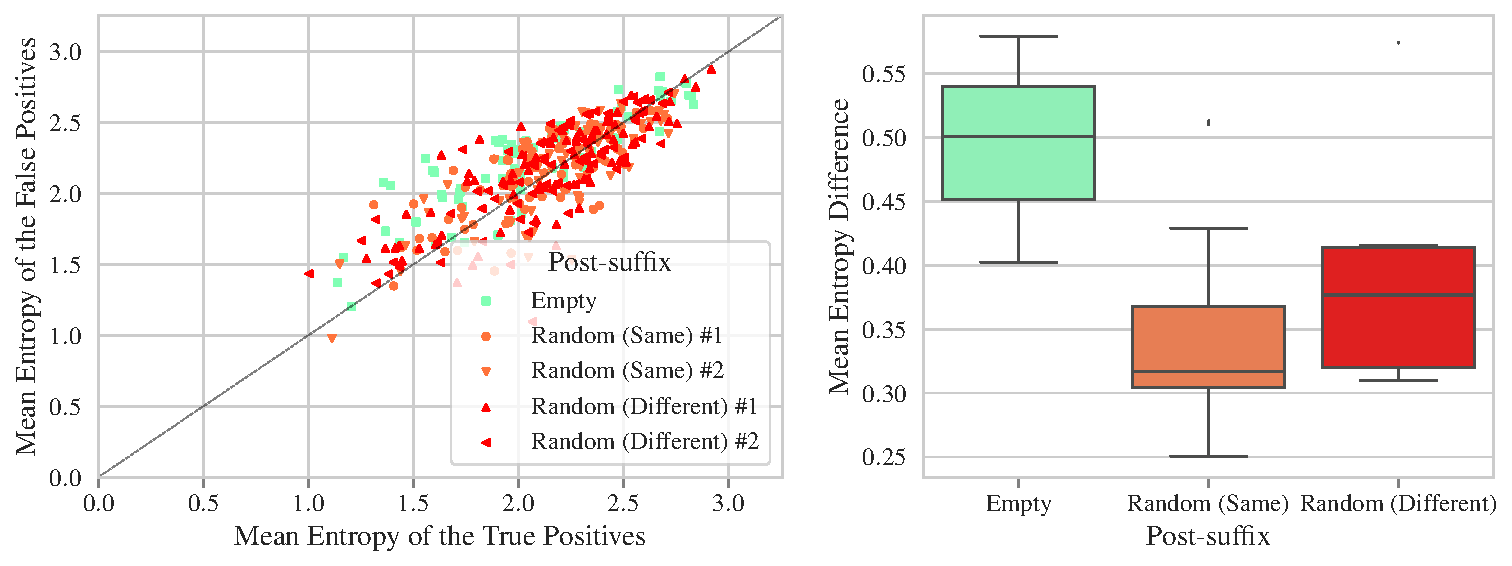
\includegraphics[width=\textwidth]{images/post-suffix_sheared_adversarial_12.pdf}
    \caption[Effect of different post-suffixes on discerning true positives from false positives with sheared images.]{Effect of different post-suffixes on discerning true positives from false positives with the sheared image. Note that the temperature here is lower, \(T = 0.012\), the points gather in the upper right corner at higher temperatures.}
    \label{fig:post-suffix_sheared_adversarial}
\end{figure}

\newpage
\section{Simulations using the Semantics Reward}
\label{sec:simulations}
% Manual ranking and entropy ranking

Using the suitable combinations of the controller and environment hyperparameters from \secref{sec:closeness-rollouts} and intuition of the regularized semantics entropy reward hyperparameters \secref{sec:improving-rewards}, we ran simulations with the semantics reward to generate creations in the environments.
We were generally able to generate meaningful creations in both environments, but the quality of the creations varied significantly.

We further investigated the effects of a few hyperparameters on the quality of the creations.
To evaluate these creations, in addition to the cumulative reward, we also asked three human evaluators to manually rank the final creations on a scale of \(1\) to \(5\) based on their apparent semantic expressiveness.
In the following parts, shown creations (in Tangram) not particularly interesting according to these rankings are desaturated to avoid visual clutter.

% B HUMAN EVALUATION
% Evaluation on tasks for which we do not have a reward function was done manually by one of the
% authors, depending on the amount of time the agent met the criteria listed in Table 2. See Figures 5
% and 6 for the raw labels obtained about the agent performance.
% We further evaluated the impact of goal-baseline regularization on the humanoid tasks that did not
% succeed in our experiments with α = 0, cf. Figure 8. In these cases, goal baseline regularization does not improve performance. Together with the results in Figure 4a, this could suggest that
% goal-baseline regularization is more useful for smaller CLIP models than for larger CLIP models.
% Alternatively, it is possible that the improvements to the reward model obtained by goal-baseline
% regularization are too small to lead to noticeable performance increases in the trained agents for the
% failing humanoid tasks. Unfortunately, a more thorough study of this was infeasible due to the cost
% associated with human evaluations.
% Our second type of human evaluation is to compute the EPIC distance of a reward model to a prelabelled set of states. To create a dataset for these evaluations, we select all checkpoints from the
% training run with the highest VLM-RM reward of the largest and most capable VLM we used. We
% then collect rollouts from each checkpoint and collect the images across all timesteps and rollouts
% into a single dataset. We then have a human labeller (again an author of this paper) label each image
% according to whether it represents the goal state or not, using the same criteria from Table 2. We
% use such a dataset for Figure 4. Figure 7 shows a more detailed breakdown of the EPIC distance for
% different model scales.

These simulations were computationally expensive and required a lot of time to run.
We were limited in our ability to fine-tune all the hyperparameters to the fullest extent, so we focused on the main few -- the regularization strengths and the effect of additional regularity reward RaIR.
We showcase the results of these analyses in the following sections.

While we ran many additional simulations to confirm our intuitions about the hyperparameters, only a few of our analyses used enough restarts with different random seeds to have enough statistical power to make justified claims.
Interesting creations from these simulations are curated in \secref{sec:gallery}\footnote{Animations and summary graphs of all the simulations and creations referenced in this thesis are available on \url{https://drive.google.com/drive/folders/1RdG86GLLujH3z6eDRIvdaczokpr8krnc} or \url{https://t.ly/49O3h}.}.

% \subsection{Evaluating Regularized Entropy Reward Formulation in Goal-Conditioned Tasks}
% \label{sec:evaluating-regularized-entropy}
% % alpha_target
% % beta_image

\subsection{Effect of Regularization Strengths}
\label{sec:alpha-beta-semantics}
% Model Search
We ran simulations with different regularization strengths to reconcile their effects with their results from the previous sections.

We find that the mid-values of the regularization strengths are the best for the performance of the controller, which is in line with the results from the ablation study in \secref{sec:reg-alpha-beta}.
\figref{fig:alpha-beta-semantics} shows the heatmap of the mean cumulative rewards for different combinations of the regularization strengths.
For standard deviations, please see \figref{fig:alpha_beta-semantics_std_rair}.

% alpha_beta-semantics_rair.pdf -- heatmap
\begin{figure}[H]
    \centering
    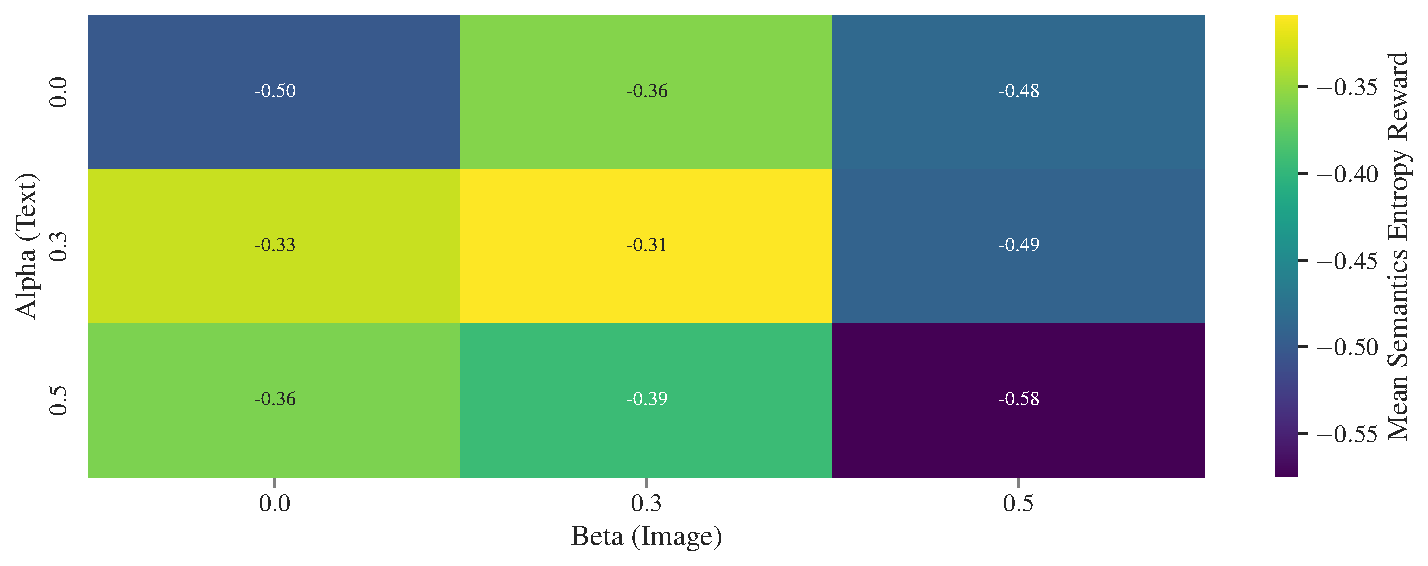
\includegraphics[width=\textwidth]{images/alpha_beta-semantics_rair.pdf}
    \caption[Performance of regularization strengths on semantics reward.]{Performance of regularization strengths on semantics reward. \(10\) seeds were used.}
    \label{fig:alpha-beta-semantics}
\end{figure}

\figref{fig:alpha-beta-trajectories} shows the effect of regularization strengths on the semantics entropy reward trajectories and \figref{fig:alpha-beta-samples} shows some samples of the creations with different regularization strengths

\begin{figure}[H]
    \centering
    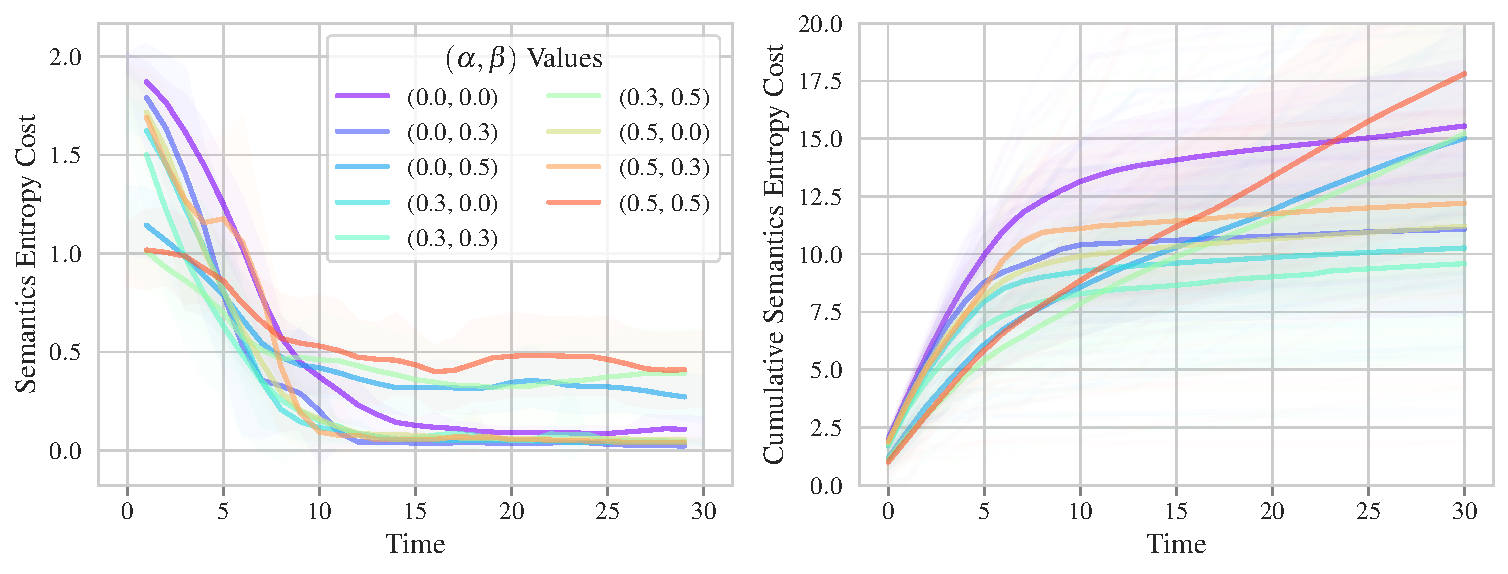
\includegraphics[width=\textwidth]{images/alpha_beta_comparison_rair.pdf}
    \caption{Effect of regularization strengths on semantics entropy reward trajectories.}
    \label{fig:alpha-beta-trajectories}
    \vspace{12pt}
    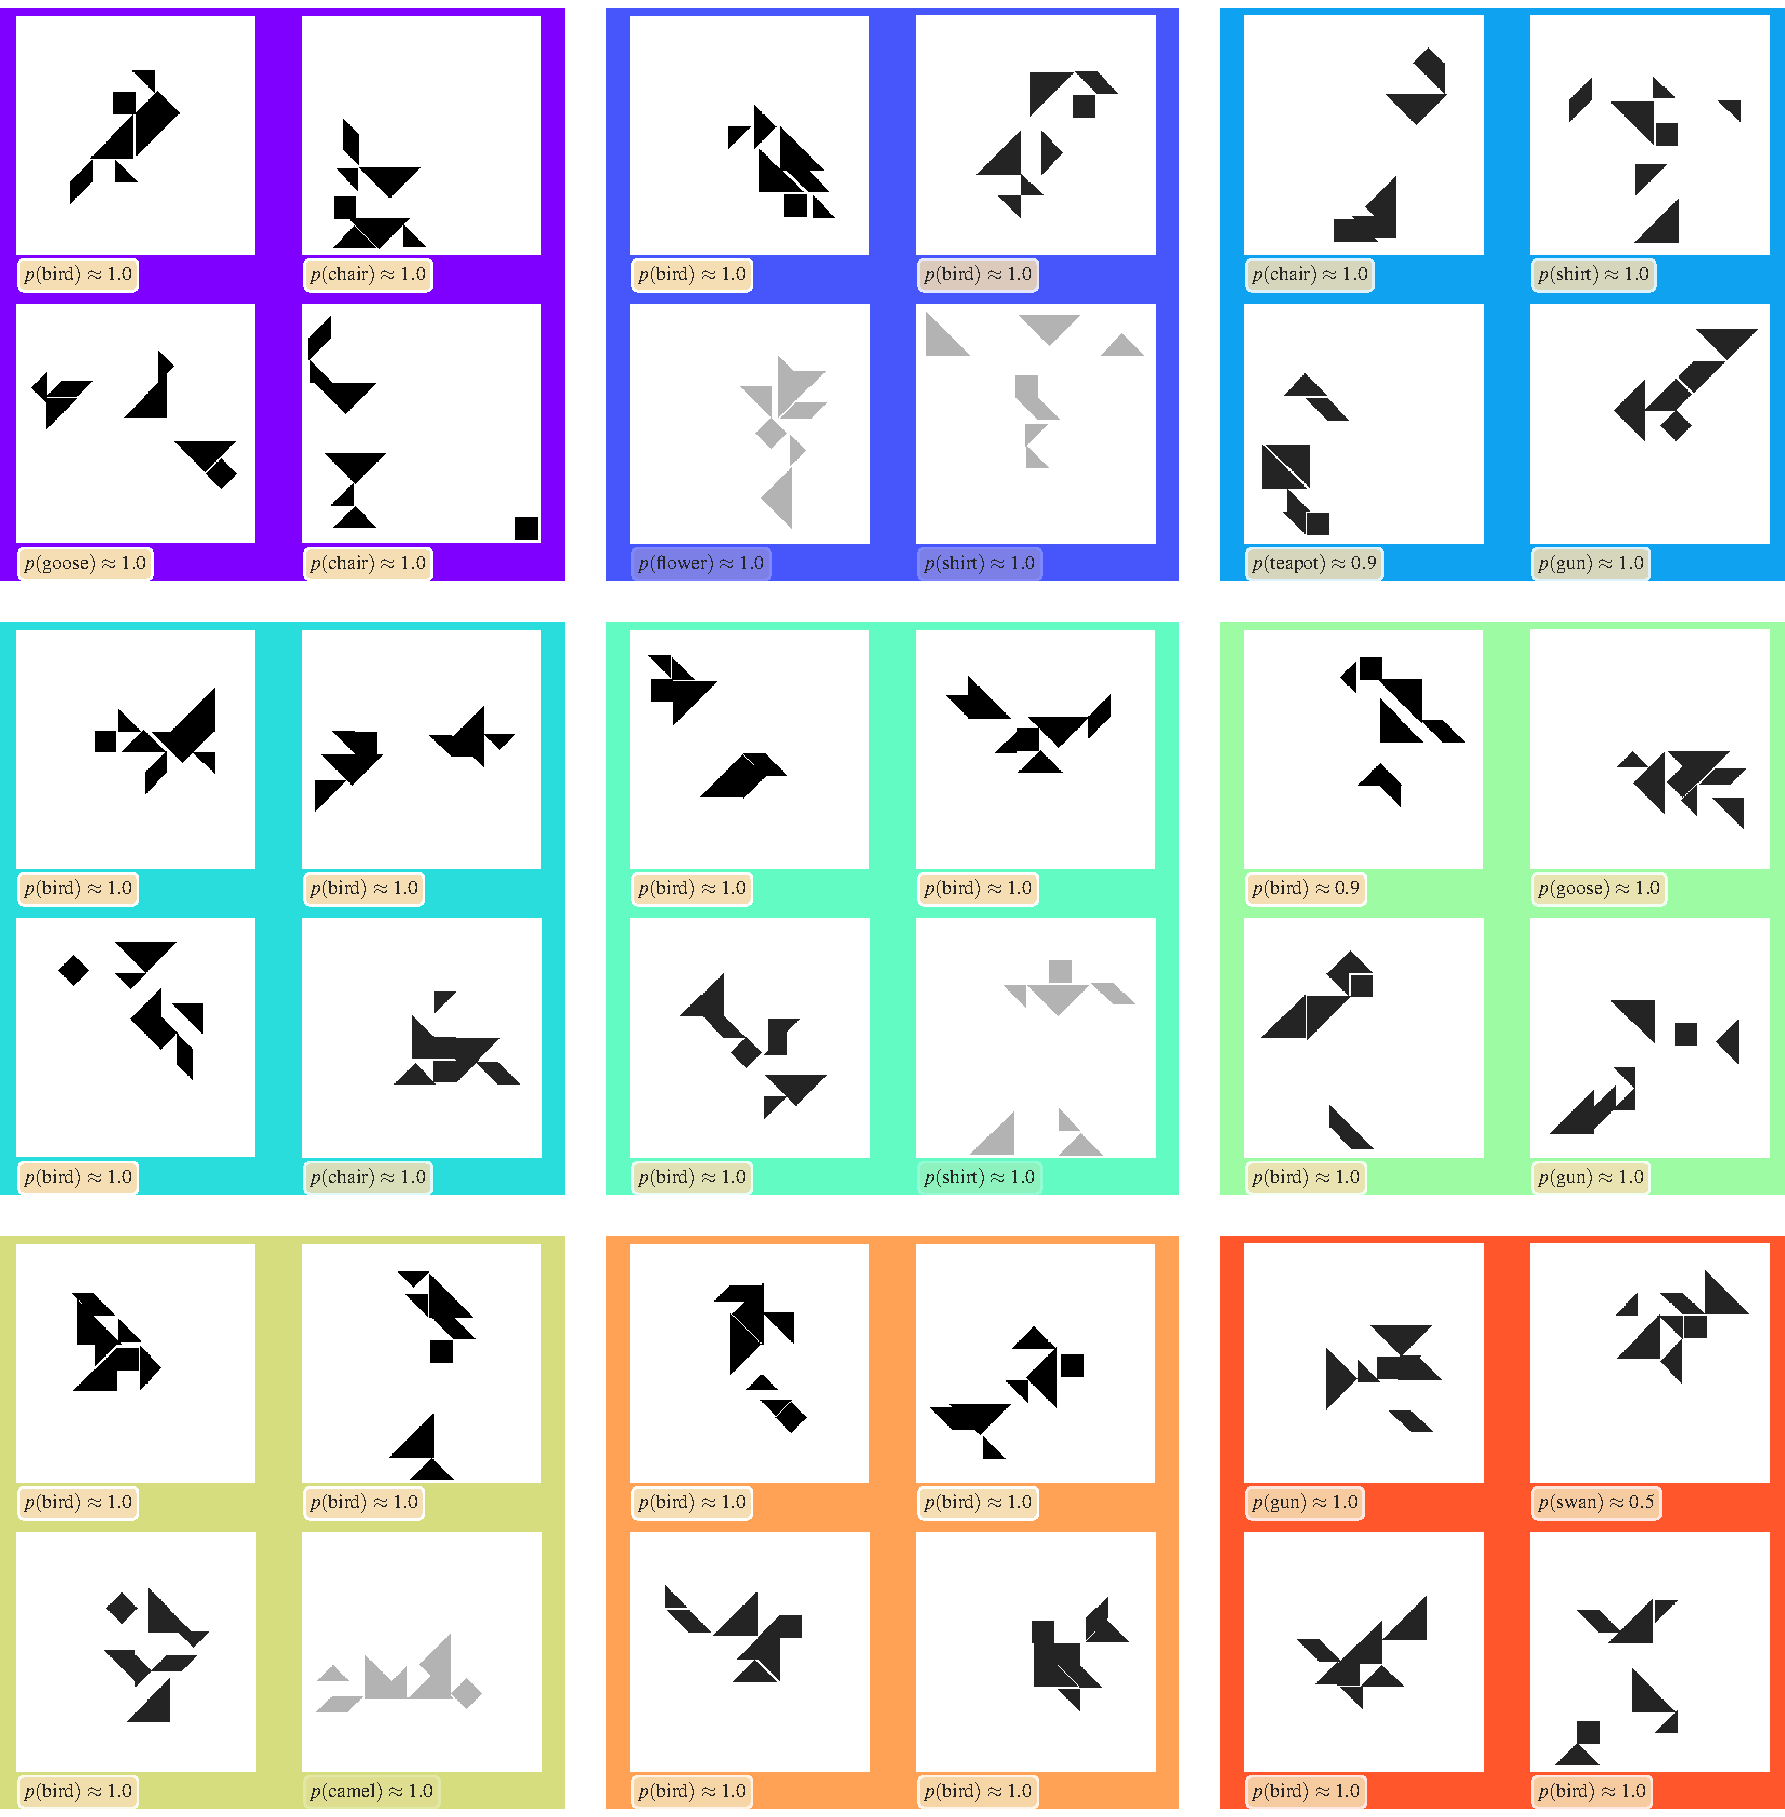
\includegraphics[width=0.8\textwidth]{images/alpha_beta_rair_samples.pdf}
    \caption{Samples of creations with different regularization strengths.}
    \label{fig:alpha-beta-samples}
\end{figure}
\todo{Explain this}

\newpage
\subsection{Effect of RaIR}
\label{sec:effect-rair}
% compression_precision
% 1 / semantics_reward_scale

Throughout our simulations, we noticed a high degree of regularity in semantic creations and a high correlation between the RaIR and the semantics entropy reward. 
Indeed, adding the structural bias from RaIR helped with grounding and coalescing the creations in more human-recognizable forms and patterns.
This was particularly helpful in the beginning of the planning as the agent starts building regular structures to bring it closer to a semantically meaningful state which is then further refined by the semantics entropy reward.
We found that creations simulated with RaIR were much more recognizable than without it.
\figref{fig:rair} shows the effect and \figref{fig:rair-samples} shows some samples of the creations with and without RaIR.

% rair_comparison.pdf
\begin{figure}[H]
    \centering
    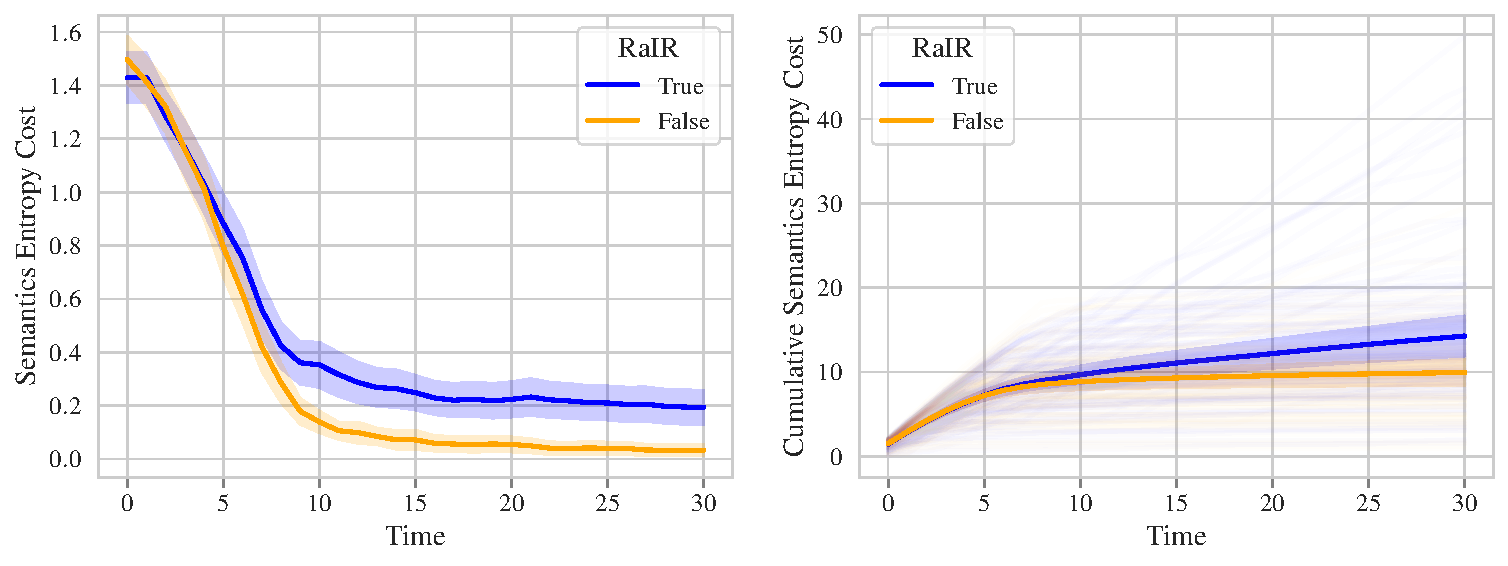
\includegraphics[width=\textwidth]{images/rair_comparison.pdf}
    \caption{Effect of RaIR on semantics entropy reward in Tangram.}
    \label{fig:rair}
    \vspace{12pt}
    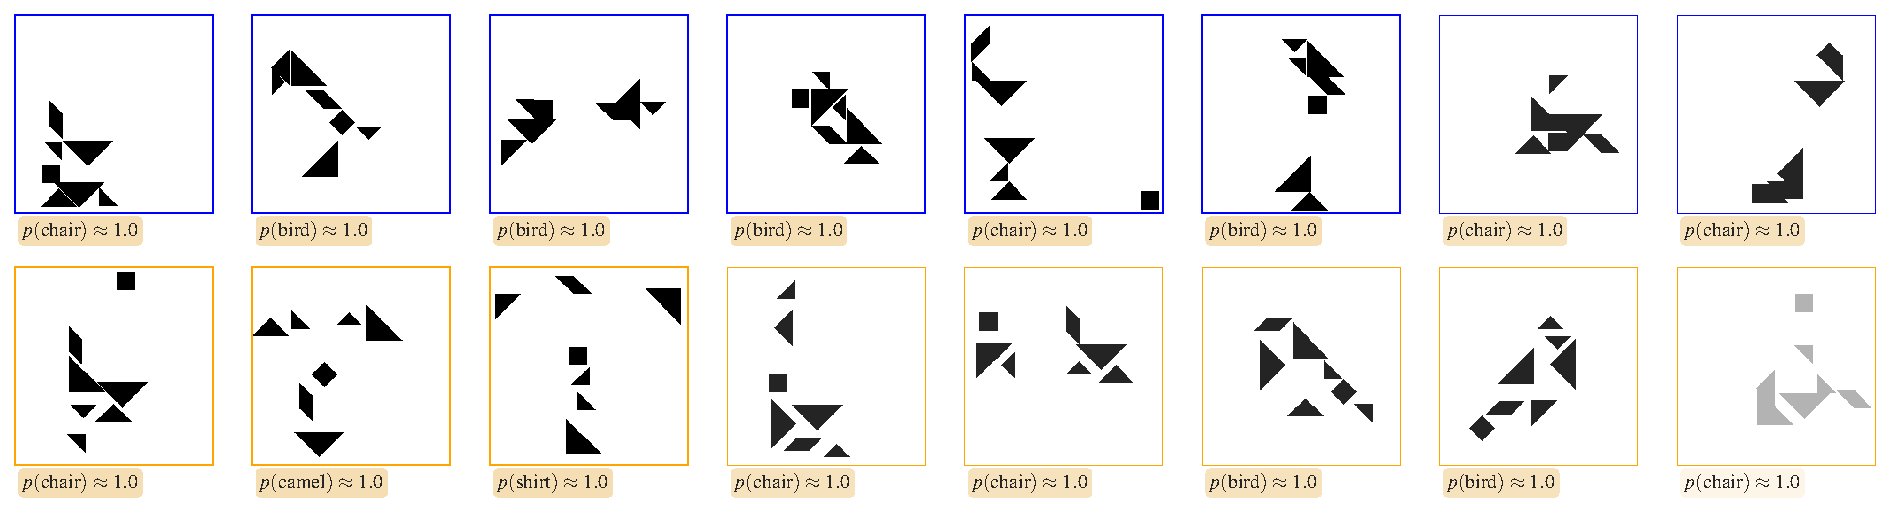
\includegraphics[width=\textwidth]{images/rair_samples.pdf}
    \caption{Samples of creations with and without RaIR.}
    \label{fig:rair-samples}
\end{figure}

\todo{talk about observations of optimizing regularity after semantics}
\todo{talk about the weight of RaIR}
\todo{Creations are neater}

\begin{figure}[H]
    \centering
    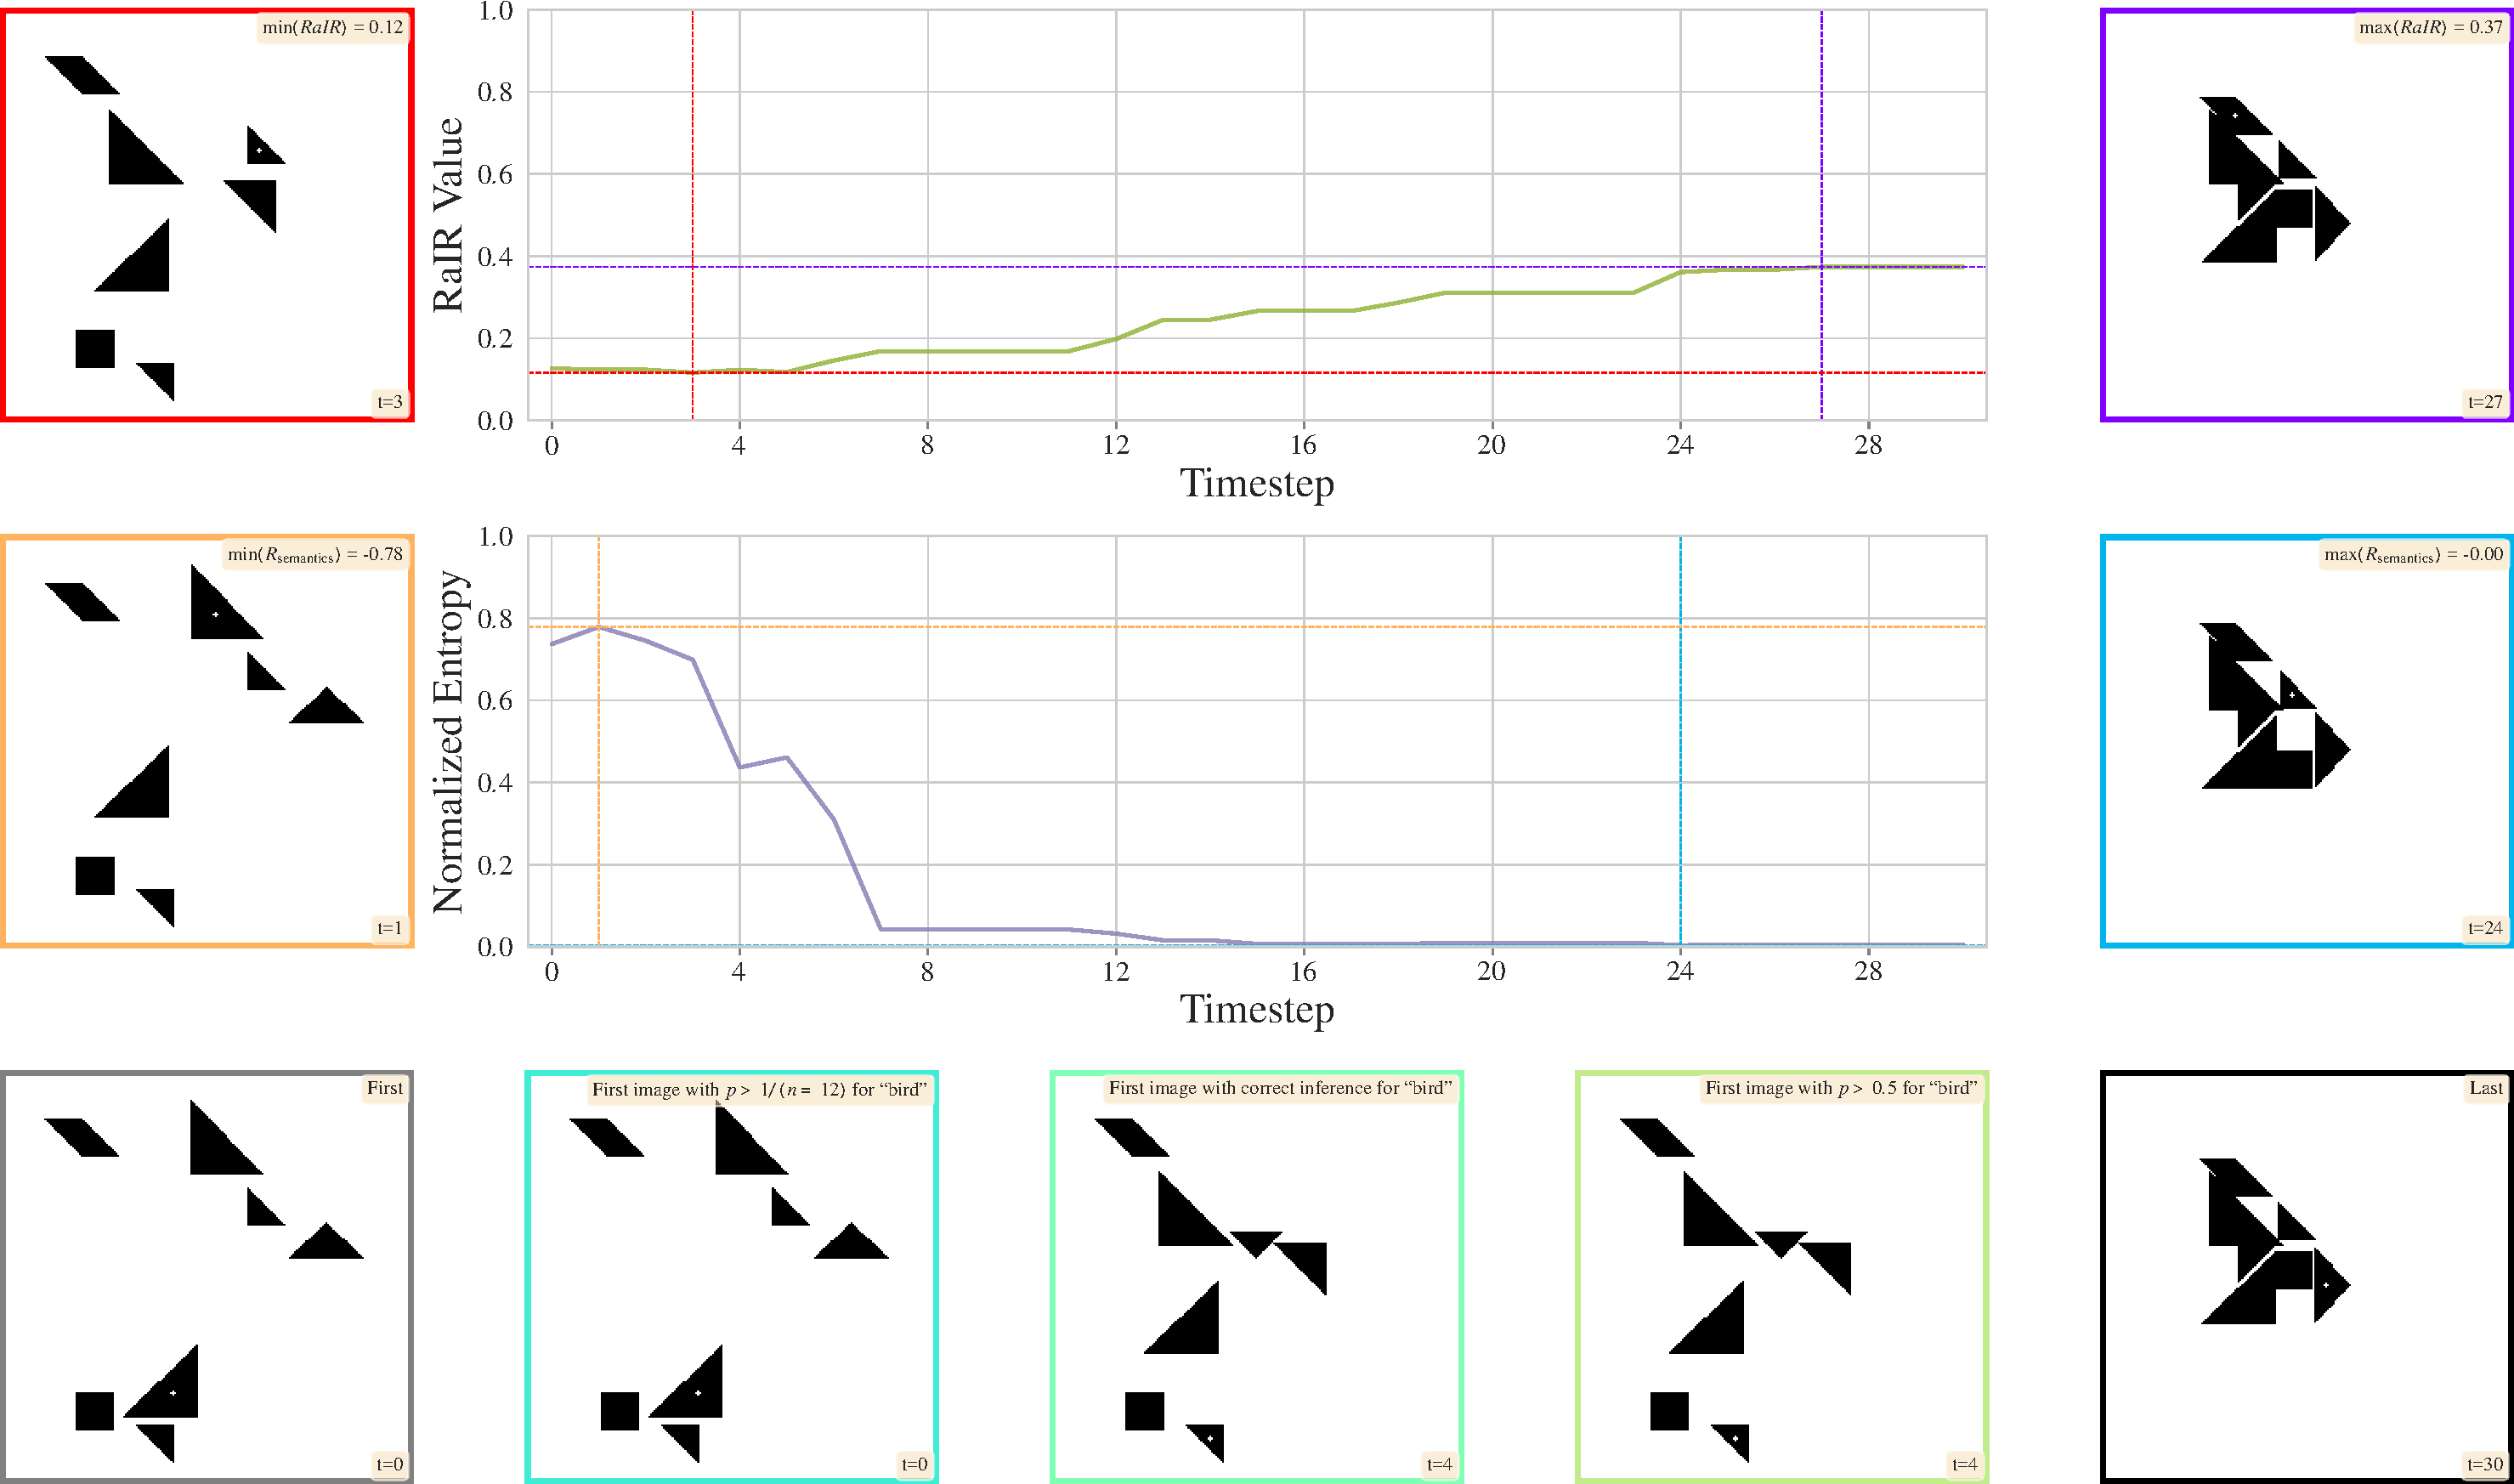
\includegraphics[width=\textwidth]{images/sim_rair_later_bird.pdf}
    \caption{Simulation on Tangram with the complete semantics reward leading to a bird creation.}
    \label{fig:sim}
\end{figure}

We also tested this in ShapeGridWorld, where the effect of RaIR was only marginal and only affected when the pixels had grayscale values.

\figref{fig:rair-color-sgw} and \figref{fig:rair-samples-color-sgw} show the effect of RaIR on ShapeGridWorld with grayscale pixels.

% rair_comparison_sgw_color.pdf
\begin{figure}[h]
    \centering
    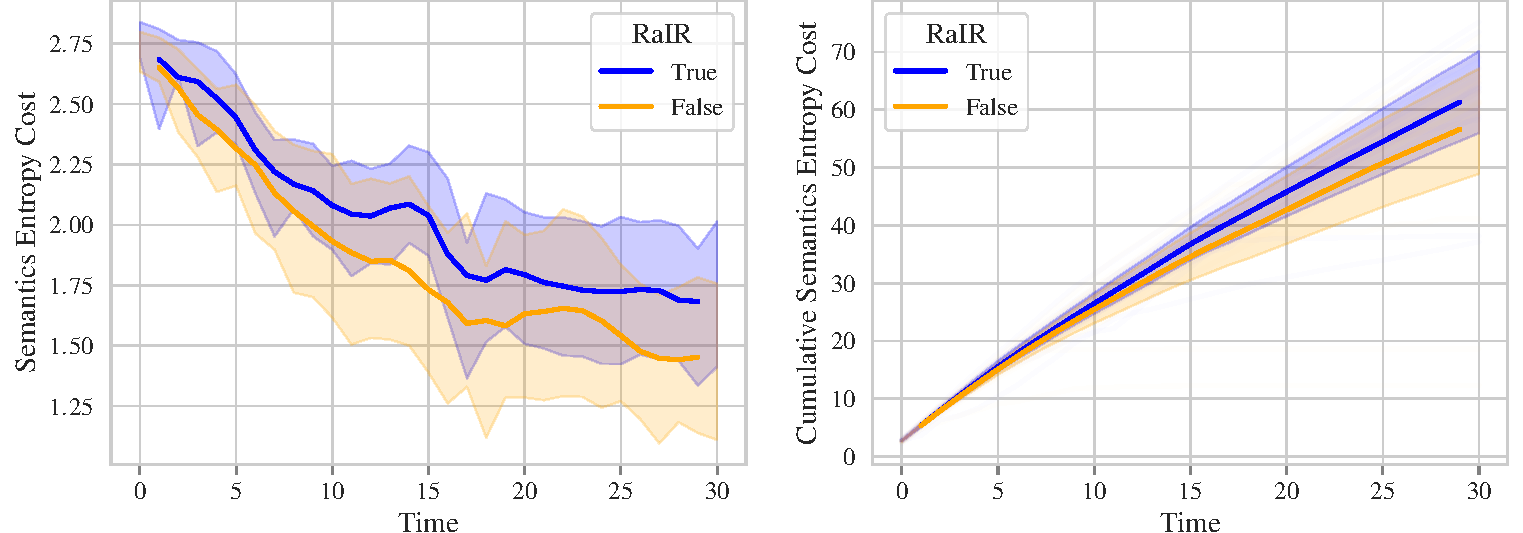
\includegraphics[width=\textwidth]{images/rair_comparison_sgw_color_cropped.pdf}
    \caption{Effect of RaIR on ShapeGridWorld with grayscale pixels.}
    \label{fig:rair-color-sgw}
    \vspace{12pt}
    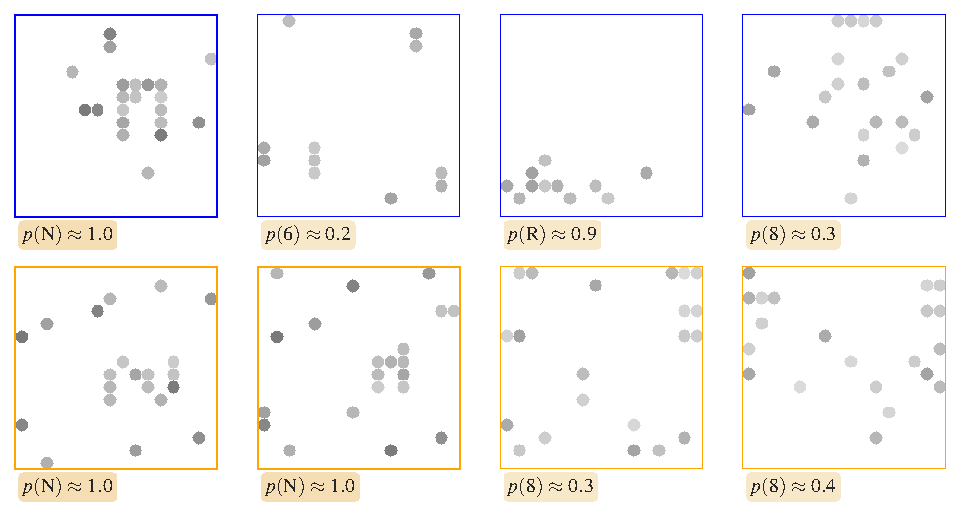
\includegraphics[width=0.5\textwidth]{images/rair_samples_sgw_color.pdf}
    \caption{Samples of creations with and without RaIR in ShapeGridWorld with grayscale pixels.}
    \label{fig:rair-samples-color-sgw}
    % rair_comparison_sgw_categories.pdf
    \vspace{12pt}
    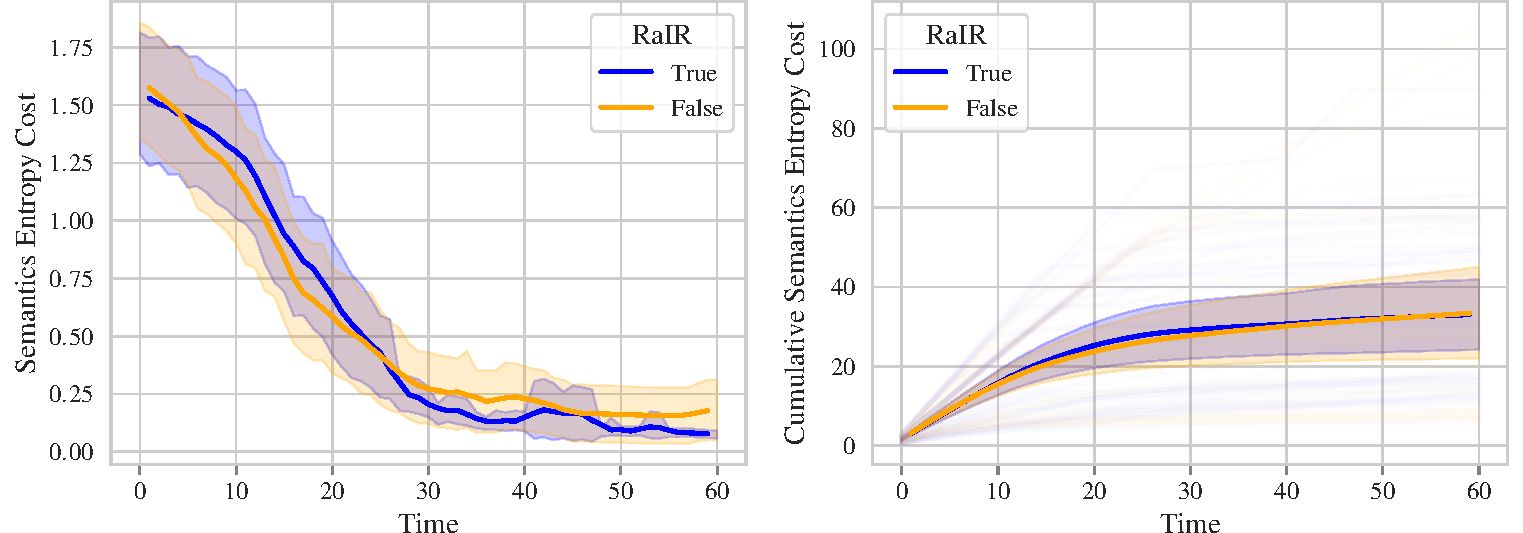
\includegraphics[width=\textwidth]{images/rair_comparison_sgw_categories_cropped.pdf}
    \caption{Effect of RaIR on ShapeGridWorld.}
    \label{fig:rair-sgw}
    \vspace{12pt}
    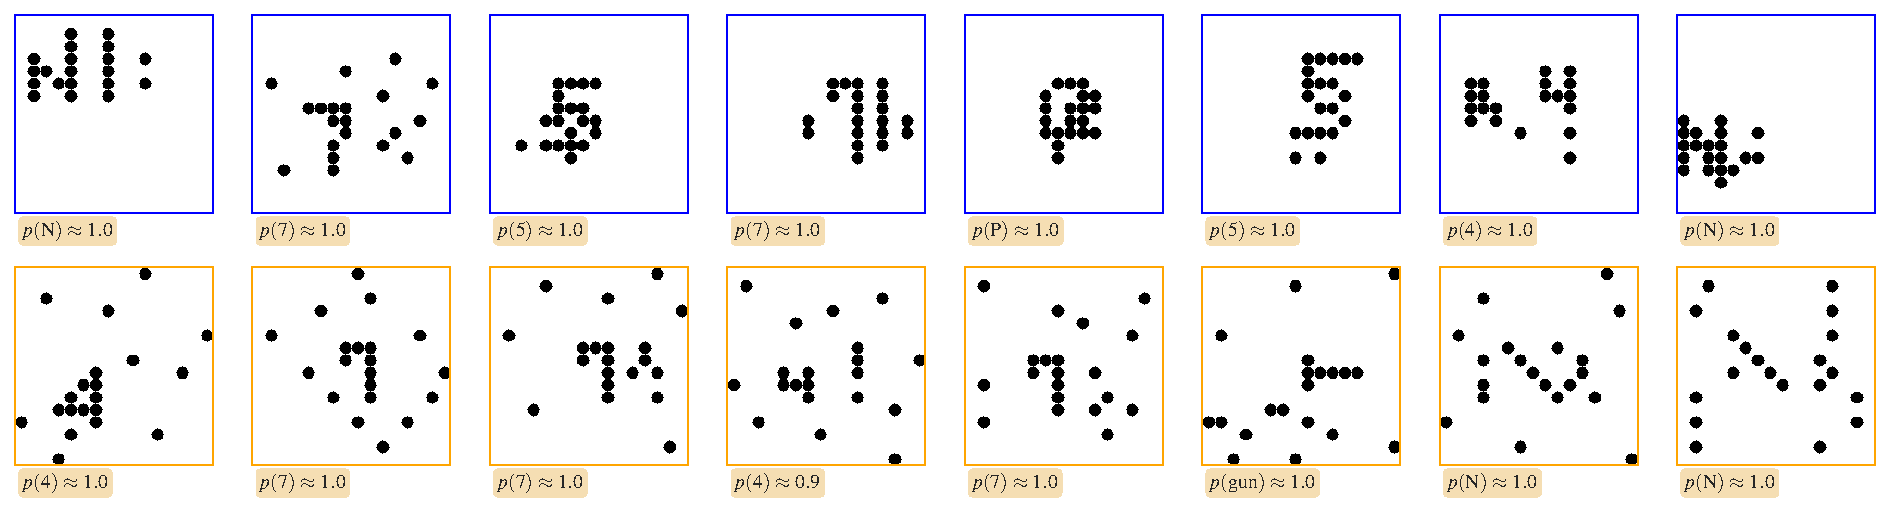
\includegraphics[width=\textwidth]{images/rair_samples_sgw_categories.pdf}
    \caption[Samples of creations with and without RaIR in ShapeGridWorld.]{Samples of creations with and without RaIR in ShapeGridWorld. % Using the \texttt{best} aggregation function.
    }
    \label{fig:rair-samples-sgw}
\end{figure}

% \subsection{Final Simulations on ShapeGridWorld}
% \label{sec:sgw-semantics}

% While we were consistently able to get good creations on Tangram, the results on ShapeGridWorld due to the many degrees of freedom were more varied.

% We ran final simulations on ShapeGridWorld with the best hyperparameters from the previous analyses.
% \figref{fig:sgw-trajectories} shows the effect of regularization strengths on the semantics entropy reward trajectories.

Results for additional simulations on ShapeGridWorld are given in \secref{sec:sgw-semantics-additional}.
